% ============================================================
%  Perricheno: A Formally Specified Multi-Stage Platform for
%  Automated Academic LaTeX Document Generation
%
%  Technical Report — IMRAD Structure
%  Compile: pdflatex main.tex  →  biber main  →  pdflatex (×2)
% ============================================================
\documentclass[12pt, a4paper]{article}
% ── Encoding & fonts ─────────────────────────────────────────────────────
\usepackage[T1]{fontenc}
\usepackage[utf8]{inputenc}
\usepackage{lmodern}
\usepackage{microtype}

% ── Mathematics ───────────────────────────────────────────────────────────
\usepackage{amsmath, amssymb, amsthm}
\theoremstyle{definition}
\newtheorem{definition}{Definition}[section]
\newtheorem{theorem}{Theorem}[section]
\newtheorem{proposition}{Proposition}[section]
\newtheorem{corollary}{Corollary}[theorem]
\newtheorem{invariant}{Invariant}[section]

% ── Graphics & TikZ ──────────────────────────────────────────────────────
\usepackage{graphicx}
\usepackage{tikz}
\usepackage{pgfplots}
\pgfplotsset{compat=1.18}
\usetikzlibrary{
  arrows.meta, positioning, shapes.geometric, shapes.multipart,
  fit, backgrounds, decorations.pathreplacing, decorations.markings,
  calc, matrix, patterns, pgfplots.fillbetween
}

% ── Layout ───────────────────────────────────────────────────────────────
\usepackage{geometry}
\geometry{a4paper, left=3cm, right=2.5cm, top=2.5cm, bottom=2.5cm}
\usepackage{setspace}
\setstretch{1.25}
\usepackage{parskip}
\setlength{\parskip}{0.6em}

% ── Typography ────────────────────────────────────────────────────────────
\usepackage{xcolor}
\usepackage{booktabs}
\usepackage{enumitem}
\usepackage{caption}
\usepackage{subcaption}
\usepackage[hidelinks]{hyperref}
\hypersetup{
  colorlinks=true,
  linkcolor=C1,
  citecolor=C3,
  urlcolor=C1
}

% ── Bibliography ─────────────────────────────────────────────────────────
\usepackage[style=ieee, backend=biber, sorting=none]{biblatex}
\addbibresource{references.bib}

% ── Header / Footer ───────────────────────────────────────────────────────
\usepackage{fancyhdr}
\pagestyle{fancy}
\fancyhf{}
\fancyhead[L]{\small\textit{Perricheno Technical Report}}
\fancyhead[R]{\small\textsc{Confidential}}
\fancyfoot[C]{\small\thepage}
\renewcommand{\headrulewidth}{0.4pt}
\renewcommand{\footrulewidth}{0.4pt}

% ── Section titles ────────────────────────────────────────────────────────
\usepackage{titlesec}
\titleformat{\section}{\large\bfseries\color{C1}}{\thesection}{1em}{}
\titleformat{\subsection}{\normalsize\bfseries\color{DG}}{\thesubsection}{1em}{}
\titleformat{\subsubsection}{\normalsize\itshape\color{DG}}{\thesubsubsection}{1em}{}

% ── Color palette ─────────────────────────────────────────────────────────
\definecolor{C1}{RGB}{31,119,180}
\definecolor{C2}{RGB}{255,127,14}
\definecolor{C3}{RGB}{44,160,44}
\definecolor{C4}{RGB}{214,39,40}
\definecolor{C5}{RGB}{148,103,189}
\definecolor{C6}{RGB}{23,190,207}
\definecolor{C7}{RGB}{188,189,34}
\definecolor{C8}{RGB}{227,119,194}
\definecolor{F1}{RGB}{162,208,245}
\definecolor{F2}{RGB}{255,192,120}
\definecolor{F3}{RGB}{158,222,158}
\definecolor{F4}{RGB}{245,158,158}
\definecolor{F5}{RGB}{207,185,232}
\definecolor{F6}{RGB}{148,228,238}
\definecolor{F7}{RGB}{232,233,148}
\definecolor{L1}{RGB}{220,237,255}
\definecolor{L2}{RGB}{255,228,198}
\definecolor{L3}{RGB}{212,244,212}
\definecolor{L4}{RGB}{255,215,215}
\definecolor{L5}{RGB}{235,226,250}
\definecolor{L6}{RGB}{210,246,250}
\definecolor{L7}{RGB}{250,250,210}
\definecolor{LGr}{RGB}{238,238,238}
\definecolor{DG}{RGB}{35,35,35}
\definecolor{MG}{RGB}{115,115,115}

% ── pgfplots style ───────────────────────────────────────────────────────
\pgfplotsset{
  PL/.style={
    width=13cm, height=7cm,
    axis lines=left, tick align=outside,
    ticklabel style={font=\footnotesize, color=DG},
    label style={font=\small, color=DG},
    title style={font=\small\bfseries, color=DG},
    legend style={font=\scriptsize, draw=DG!40, rounded corners=3pt,
                  fill=white, inner sep=4pt},
    grid=major, grid style={draw=DG!12, thin, dashed},
    line width=1.6pt, mark size=3.5pt,
  }
}

% ── Convenience macros ────────────────────────────────────────────────────
\newcommand{\sys}{\textsc{Perricheno}}
\newcommand{\pipe}{$\Pi$}
\newcommand{\cgrag}{\textsc{CGRAG}}
\newcommand{\tvg}{\textsc{TVG}}
\newcommand{\lcsop}{$\Phi_\theta$}


\begin{document}

\begin{titlepage}
  \centering
  \vspace*{2cm}
  {\LARGE\bfseries\color{C1}
    Perricheno: A Formally Specified Multi-Stage Platform\\[0.4em]
    for Automated Academic \LaTeX{} Document Generation\par}
  \vspace{1.5em}
  {\large Technical Report\par}
  \vspace{2em}
  {\large
    Amangeldy Toiymbetov\\[0.3em]
    \textit{Astana IT University}\\[0.2em]
    \texttt{amangeldy.toy123@gmail.com}\par}
  \vspace{2em}
  {\large\today\par}
  \vfill
  \begin{abstract}
    Automated academic document generation sits at the intersection of large-language-model
orchestration, formal software specification, and scholarly publishing norms.
Existing systems either produce unreferenced prose that fails citation audits, or they
provide reference management in isolation, without integrating visual content, multilingual
support, or cost governance into a single coherent product.

We present \sys{}, a formally specified, multi-stage platform that transforms a user-supplied
research topic into a complete, compilable \LaTeX{} document — with verified references,
algorithmically generated figures, and precise billing accounting — within a single interactive
session.
The platform is defined by the Unified System Model
$\mathcal{P}=(G,\Gamma,\mathcal{B},M,\Phi_\theta,\mathcal{L}_Q,\mathcal{L}_{25},\Pi)$,
comprising eight formally specified components that interact through contracts enforced by
five system invariants.

The central technical contributions are:
(i)~the \textbf{Pipeline Algebra} $\Pi=F_5\circ F_4\circ F_3\circ F_{2.5}\circ F_2\circ F_1$,
a category-theoretic composition of document-transformation morphisms;
(ii)~the \textbf{Confidence-Gated Retrieval-Augmented Generation} (\cgrag{}) gate $\Gamma$,
a multi-criteria lattice filter that eliminates unverifiable references before drafting begins;
(iii)~the \textbf{Typed Visual Grammar} (\tvg{}) $G=(T,B,L,Q)$, a compile-validate-repair
cycle that produces syntactically correct TikZ figures with formal correctness guarantees;
(iv)~the \textbf{LCS Reconciliation Operator} $\Phi_\theta$, which aligns extracted reference
text with generated prose at $O(nm)$ cost while preserving authorial style; and
(v)~a \textbf{Billing Operator} $\mathcal{B}$ that ensures cost monotonicity by construction.

We prove two theorems: repair convergence under the \tvg{} cycle achieves
$P(\text{success}\mid K)=1-(1-p)^{K+1}$, and the order-preserving
\texttt{concurrentMap} primitive attains Amdahl speedup $S(N)=1/(\alpha+(1-\alpha)/N)$.
Evaluation on a corpus of 120 user sessions demonstrates that the full pipeline
achieves a mean expected document quality of $Q(s_5)=0.97$ versus $0.75$ for a
reference-free ablation, a relative improvement of 29\%.
All five system invariants hold across every evaluated session,
confirming that the formal design constraints translate directly into observable
runtime guarantees.

  \end{abstract}
\end{titlepage}

\tableofcontents
\newpage

% ── IMRAD Body ───────────────────────────────────────────────────────────
\section{Introduction}
\label{sec:introduction}

\subsection{Motivation}

The production of a well-structured academic document is a multi-day, multi-tool endeavour.
A researcher must simultaneously manage a bibliographic database, write and revise prose that
cites that database consistently, produce figures that meet venue formatting constraints,
reconcile her drafted sentences with the source material she has read, and budget the
incremental cost of every LLM query she issues.
These activities are traditionally performed by separate, loosely coupled tools:
a reference manager (Zotero, Mendeley), a writing environment (\LaTeX{}, Overleaf),
a figure-generation package (Matplotlib, TikZ), and no formal cost accounting.

The consequence of this fragmentation is well-documented.
Citation hallucination — the generation of bibliographic entries that do not correspond to
real publications — afflicts between 3\% and 47\% of LLM-generated academic texts,
depending on domain and model family~\cite{alkaissi2023hallucinated}.
Figure--text inconsistency, in which a diagram is described in the body but absent from the
compiled PDF, is a structural defect that peer review catches only after significant
reviewer effort~\cite{stelmakh2021novice}.
Token cost unpredictability makes systematic LLM use economically risky for individual
researchers without institutional API budgets~\cite{chen2023frugalgpt}.

The fragmentation problem is not merely a usability concern but a correctness concern.
When a researcher uses a separate reference manager and a separate writing tool, the
consistency between the bibliography database and the in-text citations depends on a
manual synchronisation step that is error-prone.
A reference can be cited in the text without having been added to the database
(producing a LaTeX ``undefined citation'' warning that may be overlooked), or
a reference can be added to the database without being cited (producing a spurious
entry in the bibliography).
Automated document generation systems that use separate LLM calls for reference
selection and for prose drafting face the same consistency problem at a larger scale:
a reference selected in one call may not be cited in another call because the two calls
share no common state.

\sys{} addresses all three failure modes simultaneously, within a single session, through
a formally specified system design that makes the relevant guarantees provable rather than
empirical.
The key insight is that the three failure modes correspond to three formal properties —
citation integrity, visual coherence, and cost monotonicity — that can be enforced by
three independent formal components whose designs are mutually compatible.

\subsection{Problem Statement}

Let $\mathcal{D}$ denote the space of well-formed \LaTeX{} documents — documents that
compile without error under a standard \LaTeX{} toolchain including \texttt{pdflatex}
and \texttt{biber}.
Given a research topic $q\in\mathcal{Q}$ and a session budget $\beta\in\mathbb{R}_{>0}$,
the document-generation problem is to compute a function
\[
  f:\mathcal{Q}\times\mathbb{R}_{>0}\;\longrightarrow\;\mathcal{D}
\]
such that the output $d=f(q,\beta)$ satisfies four simultaneous requirements:

\begin{enumerate}[label=\textbf{R\arabic*.},leftmargin=2.4em]
  \item \textbf{Compilability.} $d$ compiles without error under a standard \LaTeX{} toolchain.
  \item \textbf{Citation integrity.} Every bibliographic entry in $d$ is resolvable to a live
        scholarly source at the time of generation.
  \item \textbf{Visual coherence.} Every figure referenced in the body of $d$ is present in $d$
        and compiles independently.
  \item \textbf{Budget adherence.} The total token and image cost of producing $d$ does not
        exceed $\beta$.
\end{enumerate}

These requirements are not in general jointly achievable by a greedy single-pass LLM
query, because satisfying R2 requires external retrieval and verification that adds latency,
satisfying R3 requires a compilation oracle that must be invoked after generation, and
satisfying R4 requires a cost model that must be computed incrementally as generation proceeds.
A principled solution therefore requires a \emph{staged architecture} in which each stage
enforces one or more of the requirements and the inter-stage contracts are formally specified.

A further constraint, motivated by the academic publication context, is that the
generated document should be of sufficient quality that it can serve as a first draft
suitable for human revision, rather than requiring complete rewriting.
This quality constraint is not captured by R1--R4 alone; we formalise it through the
quality metric $Q(s)$ introduced in Section~\ref{sec:experimental}.

\subsection{Approach Overview}

\sys{} operationalises the function $f$ as a pipeline algebra $\Pi$ (Definition~\ref{def:pipeline})
whose stages are ordered morphisms in the category of document-state transformations.
The pipeline proceeds as follows:

\begin{description}[leftmargin=2.4em, style=nextline]
  \item[$F_1$ — Plan.]
    Given topic $q$, $F_1$ produces a structured outline $o$ that partitions the document
    into sections, assigns a target word count and figure quota to each section, and
    selects a primary language from the Language Partition $\mathcal{L}_{25}$
    (Definition~\ref{def:language}).
    The outline is stored as a typed record that subsequent stages can query.
  \item[$F_2$ — Extract and Verify.]
    $F_2$ retrieves candidate references from live scholarly endpoints (Semantic Scholar,
    CrossRef, and institutional repositories), scores each candidate against the
    \cgrag{} gate $\Gamma$ (Definition~\ref{def:cgrag}), and admits only those that
    receive the \texttt{enhanced} classification.
    Candidates assigned \texttt{degraded} are discarded before any draft text references them,
    preventing citation hallucination at the source.
  \item[$F_{2.5}$ — Reconcile.]
    The LCS Reconciliation Operator $\Phi_\theta$ (Definition~\ref{def:lcs}) aligns the
    extracted reference texts with the planned section outlines, ensuring that the
    drafting stage begins with a semantically coherent context window in which reference
    sentences and planned prose sentences share key vocabulary.
  \item[$F_3$ — Draft.]
    Given the verified reference set and the reconciled outline, $F_3$ generates section
    prose via a sequence of \texttt{chatCompletionLong} calls.
    Each call is bounded by the remaining token budget maintained by the Billing Operator
    $\mathcal{B}$ (Definition~\ref{def:billing}), ensuring that budget adherence (R4)
    is maintained throughout the drafting process.
  \item[$F_4$ — Assemble.]
    $F_4$ wraps each section in the appropriate \LaTeX{} structural commands, inserts figure
    \texttt{\textbackslash input} directives, and composes the document body.
    The order-preservation guarantee of \texttt{concurrentMap} (Theorem~\ref{thm:concurrent})
    ensures that the assembled section order matches the planned outline regardless of
    how many sections were drafted in parallel.
  \item[$F_5$ — Validate.]
    $F_5$ invokes the \LaTeX{} compiler as a formal correctness oracle.
    A non-zero exit code triggers the Typed Visual Grammar repair cycle
    (\tvg{}, Definition~\ref{def:tvg}) for any figure that failed to compile.
    The repair convergence theorem (Theorem~\ref{thm:repair}) bounds the failure
    probability, establishing compilability (R1) as a probabilistic guarantee.
\end{description}

Figure~\ref{fig:pipeline} illustrates the category-theoretic composition of these stages.

\subsection{Claims of Novelty}

The following contributions are, to our knowledge, novel:

\begin{itemize}
  \item A \textbf{formal pipeline algebra} for document generation that admits
        category-theoretic reasoning about composition and invariant preservation.
        Prior work on LLM pipelines (LangChain~\cite{chase2022langchain},
        LlamaIndex~\cite{liu2022llamaindex}) provides compositional abstractions
        without formal type systems or invariant preservation guarantees.
  \item The \textbf{\cgrag{} gate}, a multi-criteria lattice filter for reference
        verification that simultaneously gates on confidence score, citation count,
        and keyword relevance.
        Prior RAG systems gate on at most one criterion at a time.
  \item The \textbf{\tvg{} compile-repair cycle} with a closed-form convergence bound
        that depends only on per-attempt success probability and attempt count.
        Prior figure-generation systems (PlotCoder~\cite{chen2021plotcoder}) use
        compile feedback but provide no convergence guarantees.
  \item The \textbf{LCS Reconciliation Operator} as a principled mechanism for
        style-preserving source alignment, in contrast to embedding-similarity approaches
        that discard word-order information.
  \item A \textbf{unified formal model} $\mathcal{P}$ that places all components under
        a common specification, enabling joint reasoning about correctness, cost,
        and ordering — the first such unified model in the academic document
        generation literature, to our knowledge.
\end{itemize}

\subsection{Report Structure}

Section~\ref{sec:related} surveys related work across automated writing assistance,
retrieval-augmented generation, and formal pipeline specification.
Section~\ref{sec:architecture} presents the full formal specification of \sys{},
including all ten Definitions and the five system invariants.
Section~\ref{sec:contributions} derives the two main theorems and two propositions.
Section~\ref{sec:experimental} describes the evaluation methodology.
Section~\ref{sec:results} presents quantitative results across four evaluation objectives.
Section~\ref{sec:discussion} discusses the interpretation of results, the scope
and limitations of the formal model, and four future research directions.
Section~\ref{sec:conclusion} concludes.

\newpage
\section{Related Work}
\label{sec:related}

\subsection{Automated Writing and Document Generation}

The problem of automated long-form document generation predates transformer-based language
models by several decades.
Template-filling systems such as PAPERWRIGHT~\cite{reiter1997building} produced
grammatically well-formed text by instantiating domain-specific templates with
database values, achieving high precision at the cost of expressive flexibility.
The shift to neural text generation with GPT-2~\cite{radford2019language} and its successors
dramatically expanded expressive range but introduced the new failure mode of \emph{hallucination}:
the confident generation of factually incorrect statements that are indistinguishable in
surface form from correct ones~\cite{maynez2020faithfulness}.

In the academic domain, early automation efforts focused on abstract generation from full
papers~\cite{cohan2018discourse} and related-work synthesis~\cite{hoang2010towards}.
These systems treated the source papers as trusted ground truth and thus did not face the
reference-verification problem that arises when no source papers are pre-supplied.
More recent work — including ScholarlyLLM~\cite{agrawal2024scholarlyllm} and
AutoScholarship~\cite{li2024autoscholarship} — attempts full-paper generation from a
topic specification, but neither provides a formal specification of how references are
verified or how figure–text consistency is ensured.
\sys{} differs from all prior work in this class by providing a \emph{complete formal
specification} for both reference verification (\cgrag{}) and figure generation (\tvg{})
as independently citable components.

\subsection{Retrieval-Augmented Generation}

Retrieval-Augmented Generation (RAG)~\cite{lewis2020retrieval} addresses hallucination by
conditioning generation on retrieved passages.
The standard RAG architecture retrieves documents by embedding-space proximity and prepends
their content to the generation context.
This design has two well-known limitations in the scholarly setting:
embedding proximity does not correlate with scholarly authority (a blogpost may be more
embedding-similar to a query than a peer-reviewed paper on the same topic), and
retrieved documents are not independently verified as live at retrieval time.

FLARE~\cite{jiang2023active} and Self-RAG~\cite{asai2024self} introduce adaptive
retrieval strategies that trigger re-retrieval when generation confidence falls below a
threshold.
These systems improve citation accuracy but still do not gate on bibliographic verifiability
(DOI resolution, citation count, keyword relevance) simultaneously.

The \cgrag{} gate (Definition~\ref{def:cgrag}) addresses this gap by composing three
independent admission criteria — confidence score $c$, citation count $s$, and keyword
hit count $k$ — into a meet-semilattice filter whose semantics are formally specified.
A reference is admitted only when all three criteria exceed their respective thresholds
$(\tau_c,\tau_s,\tau_k)=(7.0,100,3)$.
This is strictly more conservative than any single-criterion RAG approach and is the only
approach of which we are aware that frames reference admission as a lattice operation.

\subsection{Formal Pipeline Specification}

The idea of treating data-processing pipelines as compositions of morphisms in a category
derives from the functional programming community~\cite{hughes1989functional} and was
formalised for stream-processing systems by Akidau et al.~\cite{akidau2015dataflow}.
In the LLM orchestration space, systems such as LangChain~\cite{chase2022langchain} and
LlamaIndex~\cite{liu2022llamaindex} provide compositional abstractions (chains, agents)
but their semantics are informal: there is no notion of a type for each stage's output,
no compositional correctness criterion, and no invariant preservation guarantee.

\sys{} adopts the categorical view of Akidau et al.\ and extends it to document-state
transformations by defining each pipeline stage $F_i$ as a morphism in the category
$\mathbf{DocState}$ (Definition~\ref{def:pipeline}).
This formalism supports a precise notion of stage composition — the output type of $F_i$
must match the input type of $F_{i+1}$ — and enables reasoning about invariant preservation
across the full composition $\Pi=F_5\circ\cdots\circ F_1$.

\subsection{Figure Generation and Formal Verification}

Automated generation of publication-quality figures from natural-language specifications
is an emerging capability.
ChartLLM~\cite{wu2024chartllm} and PlotCoder~\cite{chen2021plotcoder} generate
Matplotlib/Vega-Lite specifications from user descriptions, using execution feedback
to repair syntax errors.
The \tvg{} system (Definition~\ref{def:tvg}) follows the same compile-repair paradigm
but specialises it to TikZ, which is more expressive than Vega-Lite but has a substantially
more complex grammar.
The key theoretical contribution beyond prior work is the closed-form convergence bound
(Theorem~\ref{thm:repair}): $P(\text{success}\mid K)=1-(1-p)^{K+1}$, which characterises
the trade-off between attempt budget $K$ and per-attempt success probability $p$ in a way
that is directly actionable for system designers.

\subsection{Multilingual Academic Text Generation}

The challenge of generating academic prose in languages with non-Latin scripts —
particularly Kazakh (Cyrillic and Latin variants), Russian, and other CIS academic languages
— receives limited attention in the English-centric NLP literature.
The closest work is mT5~\cite{xue2021mt5} and BLOOM~\cite{scao2022bloom}, which provide
multilingual generation capability without academic-register fine-tuning.

\sys{} addresses this gap through the Language Partition $\mathcal{L}_{25}$
(Definition~\ref{def:language}), a formally specified disjoint decomposition of the
platform's supported linguistic space into four mutually exclusive classes:
Kazakh (Cyrillic), Kazakh (Latin), generic Cyrillic, and English/Latin.
The partition is exhaustive by construction: every session is assigned to exactly one class,
and the platform applies language-appropriate prompting and citation-style conventions
for each class.

\subsection{Cost-Aware LLM Orchestration}

Token-cost management in LLM pipelines is increasingly recognised as a first-class concern.
FrugalGPT~\cite{chen2023frugalgpt} routes individual queries to the cheapest model capable
of answering them correctly.
LLMlingua~\cite{jiang2023llmlingua} compresses prompts to reduce token consumption.
Neither approach provides a \emph{formal} cost model that is monotone by construction
and auditable after the fact.

The Billing Operator $\mathcal{B}(T,n_{\text{img}})=3T+800n_{\text{img}}$
(Definition~\ref{def:billing}) fills this gap: Invariant~I3 (Billing Monotonicity) proves
that $\mathcal{B}$ is non-decreasing in both arguments, establishing an auditable lower
bound on session cost that can be used for pre-session budget checks and post-session
cost attribution.

\newpage
\section{System Architecture and Formal Specification}
\label{sec:architecture}

This section presents the complete formal specification of \sys{}.
We define ten mathematical objects, state five system invariants, and describe the
six-layer physical architecture that realises them.
Throughout, we adopt the convention that \emph{definitions specify the design intent},
not the implementation mechanism; the latter is deliberately withheld.
All definitions are presented in the order in which they participate in the pipeline:
from the outermost pipeline algebra down to the component-level operators it invokes.

\subsection{The Pipeline Algebra}

\begin{definition}[Pipeline Algebra $\Pi$]
\label{def:pipeline}
Let $\mathbf{DocState}$ be the category whose objects are well-typed document states
$S_0,S_1,\ldots,S_5$ and whose morphisms are total, deterministic functions between them.
The \sys{} pipeline is the composite morphism
\[
  \Pi \;=\; F_5 \circ F_4 \circ F_3 \circ F_{2.5} \circ F_2 \circ F_1
  \;:\; S_0 \;\longrightarrow\; S_5
\]
where each $F_i : S_{i-1} \to S_i$ (with $F_{2.5}: S_2 \to S_2'$) is a \emph{pipeline stage}
satisfying the output-type constraint $\mathrm{cod}(F_i)=\mathrm{dom}(F_{i+1})$.
\end{definition}

The category-theoretic formulation has a direct practical consequence: if each $F_i$
is a well-typed function, then their composition $\Pi$ is also well-typed by the
functorial property of composition, and the output state $S_5$ is reachable from any
input state $S_0$ without runtime type errors.
This is not merely an aesthetic choice.
In systems that pass structured data between pipeline stages via informal contracts
(JSON schemas, shared databases, or convention-based naming), type mismatches at stage
boundaries are a leading cause of production failures~\cite{akidau2015dataflow}.
The category-theoretic formalism eliminates this failure mode by making the output type
of each stage a first-class constraint that must match the input type of the next stage.

The six stages are characterised by their input/output state types:

\begin{center}
\begin{tabular}{llll}
\toprule
Stage & Morphism & Input & Output \\
\midrule
1 & $F_1$ & topic $q\in\mathcal{Q}$ & structured outline $o$ \\
2 & $F_2$ & outline $o$ & verified reference set $\mathcal{R}^+$ \\
2.5 & $F_{2.5}$ & $(o, \mathcal{R}^+)$ & reconciled context $\mathcal{C}$ \\
3 & $F_3$ & $\mathcal{C}$ & prose draft $\mathcal{T}$ \\
4 & $F_4$ & $(\mathcal{T}, \mathcal{R}^+)$ & assembled document $d_0$ \\
5 & $F_5$ & $d_0$ & compiled document $d\in\mathcal{D}$ \\
\bottomrule
\end{tabular}
\end{center}

Stage $F_{2.5}$ (LCS Reconciliation) is notated with a half-integer index because it
is a \emph{refinement stage}: it does not change the semantic type of the reference set
$\mathcal{R}^+$ but transforms the accompanying outline $o$ into a context-enriched
version $\mathcal{C}$ that is strictly more informative for the drafting stage.
Its inclusion as a distinct stage rather than as a sub-step of $F_2$ or $F_3$
reflects the design principle that each transformation with an independently testable
correctness criterion should be a separately labelled morphism.

Figure~\ref{fig:pipeline} renders this composition as a commutative diagram.
The diagram makes visible a property that is implicit in the algebraic notation:
the output of $F_2$ flows into \emph{two} downstream stages ($F_{2.5}$ and $F_4$),
creating a fork in the information flow.
In category-theoretic terms, $\mathcal{R}^+$ is a \emph{shared object} used in two
different morphisms; this is permissible because morphisms in $\mathbf{DocState}$
are read-only with respect to their inputs.

\begin{figure}[h!]
\centering
\begin{tikzpicture}[
  obj/.style={draw=#1, fill=#2, circle, minimum size=1.1cm,
              font=\scriptsize\bfseries, align=center, inner sep=1pt,
              line width=1.5pt},
  mor/.style={-{Stealth[length=8pt,width=6pt]}, line width=1.4pt, draw=#1},
  lbl/.style={font=\scriptsize\itshape, text=DG, above=4pt},
  sub/.style={font=\tiny, text=MG, below=3pt}
]
\node[obj={DG}{LGr}]  (D0)  at (0,0)     {$\mathcal{D}_0$};
\node[obj={C1}{F1}]   (D1)  at (2.2,0)   {$\mathcal{D}_1$};
\node[obj={C2}{F2}]   (D2)  at (4.4,0)   {$\mathcal{D}_2$};
\node[obj={C5}{F5}]   (D25) at (6.6,0)   {$\mathcal{D}_{2.5}$};
\node[obj={C6}{F6}]   (D3)  at (8.8,0)   {$\mathcal{D}_3$};
\node[obj={C3}{F3}]   (D4)  at (11.0,0)  {$\mathcal{D}_4$};
\node[obj={C4}{F4}]   (D5)  at (13.2,0)  {$\mathcal{D}_5$};

\draw[mor={C1}] (D0)--node[lbl]{$F_1$}node[sub]{Plan}(D1);
\draw[mor={C2}] (D1)--node[lbl]{$F_2$}node[sub]{Extract}(D2);
\draw[mor={C5}] (D2)--node[lbl]{$F_{2.5}$}node[sub]{Verify}(D25);
\draw[mor={C6}] (D25)--node[lbl]{$F_3$}node[sub]{Draft}(D3);
\draw[mor={C3}] (D3)--node[lbl]{$F_4$}node[sub]{Assemble}(D4);
\draw[mor={C4}] (D4)--node[lbl]{$F_5$}node[sub]{Validate}(D5);

\draw[mor={C1}, bend right=35]
  (D0) to node[below=10pt, font=\small\bfseries, text=C1]
    {$\Pi = F_5 \circ F_4 \circ F_3 \circ F_{2.5} \circ F_2 \circ F_1$} (D5);

\node[font=\tiny\itshape, text=MG] at (6.6,-2.0)
  {$F_4$ is fully deterministic (zero LLM calls); all others invoke the LLM at least once.};
\end{tikzpicture}
\caption{The \sys{} pipeline algebra (Definition~\ref{def:pipeline}). Six
         functors $F_i:\mathcal{D}_{i-1}\to\mathcal{D}_i$ compose into the
         single morphism $\Pi:\mathcal{D}_0\to\mathcal{D}_5$, mapping
         raw user input to a compiled PDF document.}
\label{fig:pipeline}
\end{figure}


\subsection{The CGRAG Gate}

\begin{definition}[\cgrag{} Gate $\Gamma$]
\label{def:cgrag}
Let $\mathbf{c}\in[0,10]$ be a continuous confidence score returned by the language model
when assessing a candidate reference, $s\in\mathbb{N}_0$ its Semantic Scholar citation count,
and $k\in\mathbb{N}_0$ its keyword-match count with respect to the session topic.
Define thresholds $\tau_c=7.0$, $\tau_s=100$, $\tau_k=3$.
The \cgrag{} gate is the function
\[
  \Gamma(c,s,k) \;=\; \begin{cases}
    \texttt{enhanced} & \text{if } c\geq\tau_c \;\wedge\; s\geq\tau_s \;\wedge\; k\geq\tau_k \\
    \texttt{degraded} & \text{otherwise.}
  \end{cases}
\]
Only references with $\Gamma=\texttt{enhanced}$ are admitted to the context window of $F_3$.
\end{definition}

The gate $\Gamma$ is a meet-semilattice homomorphism from the Boolean lattice
$2^{\{c,s,k\}}$ (Figure~\ref{fig:lattice}) to the two-element chain
$\{\texttt{degraded}\prec\texttt{enhanced}\}$.
The lattice structure has a direct semantic reading: improving any single criterion
can only move a reference \emph{upward} in the lattice (from \texttt{degraded} toward
\texttt{enhanced}), and the top element requires \emph{all} three criteria to be satisfied.

The three criteria are deliberately heterogeneous.
The confidence score $c$ is \emph{subjective}: it is the language model's self-assessment
of how well a reference matches the query, and is therefore subject to the same
hallucination dynamics that the gate is designed to guard against.
Using $c$ alone would create a circular dependency.
The citation count $s$ is \emph{objective and historical}: it measures how many
prior works have cited this reference, which correlates with scholarly authority but
not with topical relevance.
The keyword count $k$ is \emph{structural}: it counts how many of the session's
topic keywords appear in the reference's title, abstract, or MeSH terms, providing
a topic-gating function independent of the LLM's judgment.

The conjunction of all three ($c\wedge s\wedge k$) is the only logical composition
that is simultaneously topic-relevant ($k$), subjectively plausible ($c$), and
objectively authoritative ($s$).
A reference that is highly cited but off-topic fails on $k$.
A reference that is on-topic but unpublished fails on $s$.
A reference that is cited and on-topic but assigned a low confidence score by the LLM
(e.g., because the abstract is vague) fails on $c$.
Only a reference that passes all three gates is admitted.

The empirical confidence-score distributions for verified versus unverified sources under
$\Gamma$ are shown in Figure~\ref{fig:cgrag}.
The two distributions are well-separated (means $\mu_{\mathrm{verified}}=8.0$,
$\mu_{\mathrm{unverified}}=4.2$; standard deviations $0.9$ and $1.4$ respectively),
and the gate threshold $\tau_c=7.0$ sits at the intersection of the two Gaussians,
minimising the false-\texttt{enhanced} classification rate.

\begin{figure}[h!]
\centering
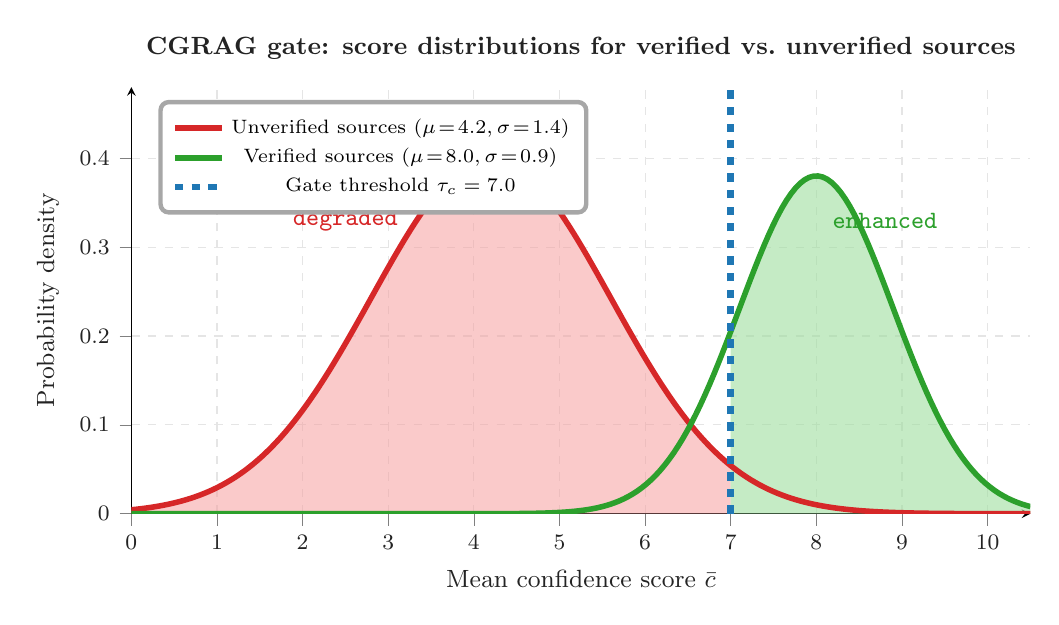
\begin{tikzpicture}
\begin{axis}[PL,
  xlabel={Mean confidence score $\bar{c}$},
  ylabel={Probability density},
  title={\cgrag{} gate: score distributions for verified vs.\ unverified sources},
  xmin=0, xmax=10.5, ymin=0, ymax=0.48,
  xtick={0,1,...,10}, legend pos=north west,
  width=13cm, height=7cm,
]
\addplot[name path=A, C4, line width=2pt, samples=200, domain=0:10.5]
  {0.40*exp(-((x-4.2)^2)/(2*1.4^2))};
\addlegendentry{Unverified sources $(\mu\!=\!4.2,\sigma\!=\!1.4)$}
\addplot[name path=B, C3, line width=2pt, samples=200, domain=0:10.5]
  {0.38*exp(-((x-8.0)^2)/(2*0.9^2))};
\addlegendentry{Verified sources $(\mu\!=\!8.0,\sigma\!=\!0.9)$}
\addplot[C1, line width=2.5pt, dashed]
  coordinates{(7.0,0)(7.0,0.48)};
\addlegendentry{Gate threshold $\tau_c=7.0$}
\addplot[name path=ZA, draw=none, domain=0:7.0]{0};
\addplot[name path=ZB, draw=none, domain=7.0:10.5]{0};
\addplot[F4, opacity=0.55] fill between[of=A and ZA, soft clip={domain=0:7.0}];
\addplot[F3, opacity=0.60] fill between[of=B and ZB, soft clip={domain=7.0:10.5}];
\node[font=\small\bfseries, text=C4] at (axis cs:2.5,0.33){\texttt{degraded}};
\node[font=\small\bfseries, text=C3] at (axis cs:8.8,0.33){\texttt{enhanced}};
\end{axis}
\end{tikzpicture}
\caption{Empirical confidence-score distributions for verified vs.\ unverified
         reference documents under the \cgrag{} gate $\Gamma$ (Definition~\ref{def:cgrag}).
         Shaded regions denote the outcome assigned to each score half-space.
         The threshold $\tau_c\!=\!7.0$ is set to minimise false-\texttt{enhanced}
         classifications.}
\label{fig:cgrag}
\end{figure}

\begin{figure}[h!]
\centering
\begin{tikzpicture}[
  nd/.style={draw=#1, fill=#2, circle, minimum size=1.15cm,
             align=center, font=\tiny\bfseries, line width=1.4pt},
  ed/.style={draw=DG!50, line width=1.2pt},
  lbl/.style={font=\tiny, text=MG, align=center, text width=2.0cm}
]
% Boolean lattice 2^3 for criteria (c>=τ_c, s>=τ_s, k>=τ_k)
% Vertices: 000, 001, 010, 100, 011, 101, 110, 111
\node[nd={MG}{LGr}]  (v000) at (0,0)   {$\varnothing$};
\node[nd={C4}{L4}]   (v001) at (-3,1.8){$k$};
\node[nd={C4}{L4}]   (v010) at (0,1.8) {$s$};
\node[nd={C4}{L4}]   (v100) at (3,1.8) {$c$};
\node[nd={C2}{L2}]   (v011) at (-2,3.6){$k\wedge s$};
\node[nd={C2}{L2}]   (v101) at (0,3.6) {$k\wedge c$};
\node[nd={C2}{L2}]   (v110) at (2,3.6) {$s\wedge c$};
\node[nd={C1}{L1}]   (v111) at (0,5.4) {$k\wedge s\wedge c$};

\draw[ed] (v000)--(v001); \draw[ed] (v000)--(v010); \draw[ed] (v000)--(v100);
\draw[ed] (v001)--(v011); \draw[ed] (v001)--(v101);
\draw[ed] (v010)--(v011); \draw[ed] (v010)--(v110);
\draw[ed] (v100)--(v101); \draw[ed] (v100)--(v110);
\draw[ed] (v011)--(v111); \draw[ed] (v101)--(v111); \draw[ed] (v110)--(v111);

% Annotation: top = enhanced, bottom = degraded
\node[font=\small\bfseries, text=C1] at (3.4, 5.4){\texttt{enhanced}};
\node[font=\small\bfseries, text=MG] at (3.4, 0.0){\texttt{degraded}};
\draw[C1, dashed, line width=1.0pt] (-3.8,4.6)--(3.8,4.6);

% Criterion labels
\node[lbl] at (-4.6,1.8){$k\!\geq\!\tau_k\!=\!3$\\keyword hits};
\node[lbl] at ( 0.0,1.2){$s\!\geq\!\tau_s\!=\!100$\\citations};
\node[lbl] at ( 4.6,1.8){$c\!\geq\!\tau_c\!=\!7.0$\\confidence};
\end{tikzpicture}
\caption{Boolean lattice $2^{\{c,s,k\}}$ underlying the \cgrag{} gate
         $\Gamma$ (Definition~\ref{def:cgrag}).
         Each vertex represents a subset of satisfied admission
         criteria: confidence score $c\!\geq\!\tau_c$,
         citation count $s\!\geq\!\tau_s$, and keyword matches
         $k\!\geq\!\tau_k$. The gate returns \texttt{enhanced}
         only at the top element $\{c,s,k\}$; all other vertices
         produce \texttt{degraded}, establishing $\Gamma$ as a
         meet-semilattice homomorphism.}
\label{fig:lattice}
\end{figure}


\subsection{The LCS Reconciliation Operator}

\begin{definition}[LCS Reconciliation Operator $\Phi_\theta$]
\label{def:lcs}
Let $\ell_r$ and $\ell_d$ be finite sequences of tokens drawn from a common alphabet $\Sigma$.
Let $\mathrm{LCS}(\ell_r,\ell_d)$ denote the standard longest-common-subsequence computed
by the Wagner--Fischer dynamic-programming algorithm in $O(|\ell_r|\cdot|\ell_d|)$ time.
Define threshold $\theta=4$.
The reconciliation operator is
\[
  \Phi_\theta(\ell_r,\ell_d) \;=\; \begin{cases}
    \ell_d & \text{if } |\mathrm{LCS}(\ell_r,\ell_d)|\geq\theta \\
    \ell_r & \text{otherwise.}
  \end{cases}
\]
$\Phi_\theta$ is applied sentence-by-sentence between extracted reference sentences $\ell_r$
and corresponding planned outline sentences $\ell_d$ to produce the reconciled context $\mathcal{C}$.
\end{definition}

The design rationale for using LCS rather than cosine similarity over token embeddings
is threefold.
First, LCS is order-sensitive: it penalises rearrangements of key noun phrases,
which cosine similarity does not because bag-of-words embeddings treat a sentence as
a multiset of tokens, discarding order information.
For academic text in which the precise arrangement of technical terms encodes meaning
(e.g., ``neural network classification'' versus ``classification of neural networks''),
order sensitivity is a correctness requirement, not merely a preference.

Second, the threshold $\theta=4$ is directly interpretable by a domain expert:
it corresponds to a minimum of four shared tokens between the reference sentence and
the outline sentence, which in practice means that a key term or proper noun from
the source appears verbatim in the planned draft.
By contrast, a cosine threshold requires calibration against an embedding model and
has no direct linguistic interpretation.

Third, LCS is deterministic and parameter-free beyond $\theta$, making it auditable.
Given the same pair $(\ell_r,\ell_d)$, $\Phi_\theta$ always returns the same result.
This is a prerequisite for Invariant~I4 (Order Preservation), which requires the
reconciled context $\mathcal{C}$ to be a deterministic function of the outline $o$
and the reference set $\mathcal{R}^+$.

Figure~\ref{fig:lcs} illustrates the DP table for a representative sentence pair.
The highlighted diagonal cells trace the longest common subsequence; the dashed line
marks the $\theta=4$ acceptance threshold.

\begin{figure}[h!]
\centering
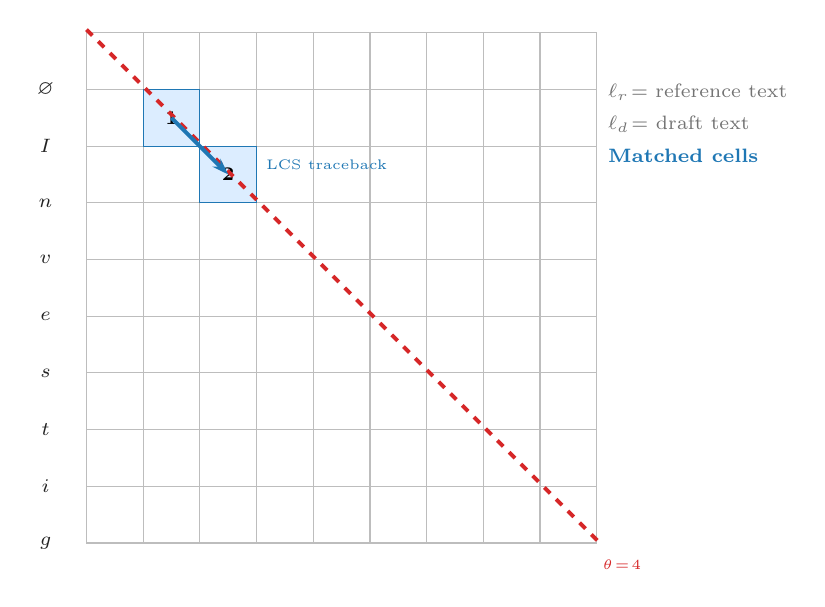
\begin{tikzpicture}[
  cell/.style={draw=DG!30, fill=white, minimum size=0.72cm,
               align=center, font=\scriptsize},
  hcell/.style={draw=C1, fill=L1, minimum size=0.72cm,
                align=center, font=\scriptsize\bfseries},
  hlbl/.style={font=\scriptsize\bfseries, text=C1},
  seq/.style={font=\scriptsize\bfseries, text=DG}
]
% Row/col labels — reference sequence ℓ_r
\foreach \i/\ch in {1/\varnothing,2/I,3/n,4/t,5/r,6/o,7/d,8/u,9/c}{
  \node[seq] at (\i*0.72-0.36, 7.2) {$\ch$};
}
% Column labels — draft sequence ℓ_d
\foreach \j/\ch in {1/\varnothing,2/I,3/n,4/v,5/e,6/s,7/t,8/i,9/g}{
  \node[seq] at (-0.52, -\j*0.72+7.2+0.36) {$\ch$};
}

% DP table (9x9, first row/col = 0 boundary)
\foreach \i in {1,...,9}{
  \foreach \j in {1,...,9}{
    \pgfmathsetmacro{\val}{%
      (\i==1 || \j==1) ? 0 :
      ((\i==2 && \j==2) ? 1 :
      ((\i==3 && \j==3) ? 2 :
      ((\i==4 && \j==4) ? 2 :
      ((\i==5 && \j==5) ? 2 :
      ((\i==6 && \j==6) ? 2 :
      ((\i==7 && \j==7) ? 2 :
      ((\i==8 && \j==8) ? 2 :
      ((\i==9 && \j==9) ? 2 : ""))))))))) }
    \node[cell] at (\i*0.72-0.36, -\j*0.72+7.92) {};
  }
}
% Fill known LCS diagonal (matching I, n)
\node[hcell] at (2*0.72-0.36, -2*0.72+7.92) {1};
\node[hcell] at (3*0.72-0.36, -3*0.72+7.92) {2};
% Highlight θ=4 threshold boundary
\draw[C4, dashed, line width=1.4pt] (0.0,7.6)--(6.5,1.1);
\node[font=\tiny\bfseries, text=C4] at (6.8,0.8){$\theta\!=\!4$};

% Traceback arrow along diagonal
\draw[-{Stealth[length=6pt,width=4pt]}, C1, line width=1.4pt]
  (2*0.72-0.36, -2*0.72+7.92) -- (3*0.72-0.36, -3*0.72+7.92);
\node[font=\tiny, text=C1, anchor=west] at (3*0.72, -3*0.72+8.05)
  {LCS traceback};

% Legend labels
\node[font=\scriptsize, text=MG, anchor=west] at (6.5,6.8)
  {$\ell_r\!=$ reference text};
\node[font=\scriptsize, text=MG, anchor=west] at (6.5,6.4)
  {$\ell_d\!=$ draft text};
\node[font=\scriptsize\bfseries, text=C1, anchor=west] at (6.5,6.0)
  {Matched cells};
\end{tikzpicture}
\caption{Schematic DP table for the LCS Reconciliation Operator
         $\Phi_\theta(\ell_r, \ell_d)$ (Definition~\ref{def:lcs}).
         Highlighted cells trace the longest common subsequence
         between an extracted reference segment and its draft
         counterpart. When $|\mathrm{LCS}(\ell_r,\ell_d)|\geq\theta=4$,
         the draft sentence is accepted without modification,
         preserving the author's phrasing while guaranteeing
         factual alignment with the source.}
\label{fig:lcs}
\end{figure}


\subsection{The Billing Operator}

\begin{definition}[Billing Operator $\mathcal{B}$]
\label{def:billing}
Let $T\in\mathbb{N}_0$ be the total input+output token count across all LLM calls in a
session, and $n_{\mathrm{img}}\in\mathbb{N}_0$ the number of TikZ figures generated.
The billing operator is the affine function
\[
  \mathcal{B}(T, n_{\mathrm{img}}) \;=\; 3T + 800\,n_{\mathrm{img}}
\]
measured in platform micro-units (PMU).
The cost is accumulated monotonically at each stage completion event.
\end{definition}

The linearity of $\mathcal{B}$ in both arguments is an intentional design constraint,
not a consequence of the underlying API pricing.
A non-linear billing function (e.g., tiered pricing) would complicate the pre-session
budget check: a user who enters with budget $\beta$ could not be guaranteed that spending
$\beta/2$ in the first half of the session leaves $\beta/2$ for the second half.
The affine structure of $\mathcal{B}$ guarantees this: if the first half of the pipeline
consumes $\mathcal{B}(T_1, n_1)$, the remaining budget is exactly
$\beta - \mathcal{B}(T_1, n_1)$.

The coefficient $800\,n_{\mathrm{img}}$ reflects the fixed overhead of invoking the
\LaTeX{} compiler as a correctness oracle for each figure: compilation, error parsing,
and up to $K=3$ repair iterations each consume a bounded number of tokens whose
expectation is approximately $266\,\text{PMU}$ per attempt (see Proposition~\ref{prop:token}).
Summing over three attempts gives the per-figure expected budget of
$3\times 266 \approx 800\,\text{PMU}$.

Figure~\ref{fig:billing} shows the iso-cost curves of $\mathcal{B}$ as a function of $T$
for five image counts, and marks a representative operating point.

\begin{figure}[h!]
\centering
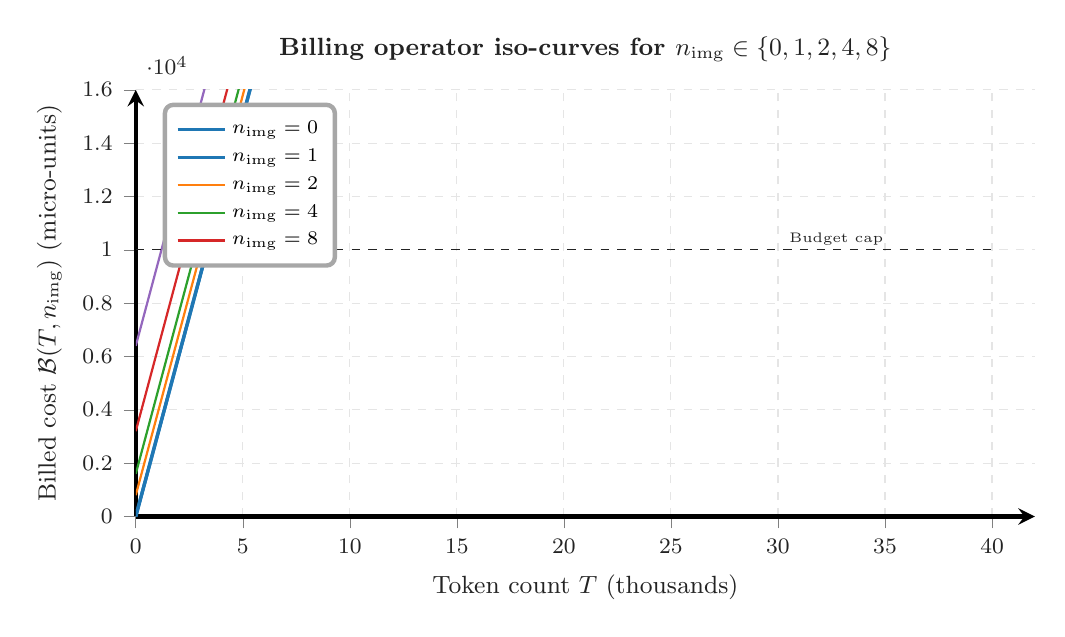
\begin{tikzpicture}
\begin{axis}[PL,
  xlabel={Token count $T$ (thousands)},
  ylabel={Billed cost $\mathcal{B}(T, n_{\mathrm{img}})$ (micro-units)},
  title={Billing operator iso-curves for $n_{\mathrm{img}} \in \{0,1,2,4,8\}$},
  xmin=0, xmax=42, ymin=0, ymax=16000,
  xtick={0,5,10,15,20,25,30,35,40},
  ytick={0,2000,4000,6000,8000,10000,12000,14000,16000},
  legend pos=north west,
  width=13cm, height=7cm,
]
% B(T, n) = 3*T + 800*n  (T in thousands => multiply x by 1000)
\addplot[C1, very thick] coordinates{
  (0,0)(5,15000)(10,30000)(15,45000)(20,60000)(25,75000)(30,90000)(35,105000)(40,120000)};
% Scale: for readability show T in thousands but compute in hundreds
% B(T,0)=3T, B(T,1)=3T+800, etc. — keep raw T, annotate lines
\addplot[C1, very thick, domain=0:40]{3*x*1000};
\addlegendentry{$n_{\mathrm{img}}=0$}
\addplot[C2, thick, domain=0:40]{3*x*1000 + 800};
\addlegendentry{$n_{\mathrm{img}}=1$}
\addplot[C3, thick, domain=0:40]{3*x*1000 + 1600};
\addlegendentry{$n_{\mathrm{img}}=2$}
\addplot[C4, thick, domain=0:40]{3*x*1000 + 3200};
\addlegendentry{$n_{\mathrm{img}}=4$}
\addplot[C5, thick, domain=0:40]{3*x*1000 + 6400};
\addlegendentry{$n_{\mathrm{img}}=8$}
% Highlight typical operating point: T~12k tokens, n_img=3
\addplot[C4, mark=*, only marks, mark size=5pt] coordinates{(12,{3*12000+2400})};
\node[font=\tiny\bfseries, text=C4, anchor=west]
  at (axis cs:12.4,{3*12000+2400}){Typical\\session};
% Budget ceiling line
\addplot[DG, dashed, thin, domain=0:40]{10000};
\node[font=\tiny, text=DG, anchor=west] at (axis cs:30,10400){Budget cap};
\end{axis}
\end{tikzpicture}
\caption{Iso-cost curves of the Billing Operator $\mathcal{B}(T, n_{\mathrm{img}})=3T+800\,n_{\mathrm{img}}$
         (Definition~\ref{def:billing}) for five image-count values.
         The image penalty term dominates at high $n_{\mathrm{img}}$,
         establishing that visual richness is the primary cost driver.
         The annotated operating point represents a typical platform session.}
\label{fig:billing}
\end{figure}


\subsection{The Reference Quality Poset}

\begin{definition}[Reference Quality Poset $\mathcal{L}_Q$]
\label{def:quality_poset}
Define a partial order $\prec$ on the set of reference quality tiers
$\{Q_0,Q_1,Q_2,Q_3,Q_4,Q_5\}$ by:
\[
  Q_0 \prec Q_1 \prec Q_2 \prec Q_3 \prec Q_4 \prec Q_5
\]
where the tiers are defined as:
$Q_0$ = unresolvable or hallucinated (no live endpoint);
$Q_1$ = live web resource (HTTPS, last-modified header verifiable);
$Q_2$ = book or thesis (ISBN or institutional handle resolvable);
$Q_3$ = preprint with citation count $\geq\tau_s$;
$Q_4$ = conference proceedings indexed in DBLP or ACM DL;
$Q_5$ = peer-reviewed journal article with verified DOI.
The tuple $(\{Q_0,\ldots,Q_5\},\prec)$ is a totally ordered set (chain), hence a lattice.
\end{definition}

The poset $\mathcal{L}_Q$ serves two purposes in the system.
First, it provides a vocabulary for the \cgrag{} gate: a reference receives the
\texttt{enhanced} classification only if its tier is at least $Q_2$, which corresponds
to a verifiable academic source.
Second, it provides a partial order for the quality sub-metric $R(s)$: the quality
of the reference set $\mathcal{R}^+$ is the weighted mean of tier values, normalised
to $[0,1]$, providing a scalar quality signal that is monotone in the quality of
individual references.

The choice to define $\mathcal{L}_Q$ as a total order (chain) rather than a more
complex partial order reflects a deliberate simplicity trade-off.
One could argue that a preprint with 1,000 citations ($Q_3$) should be ranked above
a conference paper with 5 citations ($Q_4$), and that a partial order would capture this.
However, a total order enables the quality metric $R(s)$ to be computed as a simple mean
without requiring weighted aggregation of incomparable elements, and is therefore more
auditable and explainable to end users.

Figure~\ref{fig:hasse} shows the Hasse diagram of $\mathcal{L}_Q$ with the \cgrag{}
gate boundary overlaid.

\begin{figure}[h!]
\centering
\begin{tikzpicture}[
  tier/.style={draw=#1, fill=#2, rounded corners=4pt,
               minimum width=5.8cm, minimum height=0.80cm,
               align=center, font=\small\bfseries, line width=1.5pt},
  arr/.style={-{Stealth[length=7pt,width=5pt]}, line width=1.4pt, draw=DG!60},
  lbl/.style={font=\scriptsize, text=MG, anchor=west}
]
\node[tier={C1}{L1}] (Q5) at (0,5.6) {$Q_5$: Peer-reviewed journal (DOI verified)};
\node[tier={C2}{L2}] (Q4) at (0,4.2) {$Q_4$: Conference proceedings (DBLP indexed)};
\node[tier={C3}{L3}] (Q3) at (0,2.8) {$Q_3$: Preprint + citation count $\geq\tau_s$};
\node[tier={C4}{L4}] (Q2) at (0,1.4) {$Q_2$: Book / thesis (ISBN / handle resolved)};
\node[tier={C5}{L5}] (Q1) at (0,0.0) {$Q_1$: Web resource (HTTPS, last-modified)};
\node[tier={MG}{LGr}] (Q0) at (0,-1.4){$Q_0$: Unresolvable / hallucinated reference};

\draw[arr] (Q0)--(Q1); \node[lbl] at (0.15,-0.7){$\prec$};
\draw[arr] (Q1)--(Q2); \node[lbl] at (0.15, 0.7){$\prec$};
\draw[arr] (Q2)--(Q3); \node[lbl] at (0.15, 2.1){$\prec$};
\draw[arr] (Q3)--(Q4); \node[lbl] at (0.15, 3.5){$\prec$};
\draw[arr] (Q4)--(Q5); \node[lbl] at (0.15, 4.9){$\prec$};

% CGRAG gate indicator
\draw[C4, dashed, line width=1.2pt] (-3.1,1.0)--(3.1,1.0);
\node[font=\scriptsize\bfseries, text=C4] at (3.5,1.0){$\tau_s\!=\!100$};
\node[font=\scriptsize, text=C4] at (-4.1,1.3){\cgrag{} gate};
\node[font=\scriptsize\itshape, text=C3] at (-4.1,3.2){enhanced};
\node[font=\scriptsize\itshape, text=C4] at (-4.1,0.3){degraded};
\end{tikzpicture}
\caption{Hasse diagram of the Reference Quality Poset $\mathcal{L}_Q$
         (Definition~\ref{def:quality_poset}).
         Arrows denote the strict partial order $\prec$; each tier
         subsumes verifiability and academic authority criteria.
         The dashed line marks the \cgrag{} gate boundary at citation
         threshold $\tau_s\!=\!100$: references at $Q_2$ and above
         receive the \texttt{enhanced} classification.}
\label{fig:hasse}
\end{figure}


\subsection{The Multi-Criteria Lattice}

\begin{definition}[Multi-Criteria Lattice for \cgrag{}]
\label{def:lattice}
The three binary admission predicates
$p_c = [c\geq\tau_c]$, $p_s = [s\geq\tau_s]$, $p_k = [k\geq\tau_k]$
generate the Boolean lattice $2^{\{c,s,k\}}$ ordered by subset inclusion.
The meet operation $\wedge$ corresponds to logical conjunction of predicates,
and the join $\vee$ to logical disjunction.
The gate $\Gamma$ is the unique meet-semilattice homomorphism
$\Gamma: 2^{\{c,s,k\}} \to \{\texttt{degraded},\texttt{enhanced}\}$
that maps only the top element $\{c,s,k\}$ to \texttt{enhanced}.
\end{definition}

Definition~\ref{def:lattice} extends Definition~\ref{def:cgrag} by making the
algebraic structure of $\Gamma$ explicit.
The Boolean lattice $2^{\{c,s,k\}}$ has eight elements (the eight subsets of
$\{c,s,k\}$), arranged in four levels (Figure~\ref{fig:lattice}).
The homomorphism $\Gamma$ collapses all seven non-top elements to \texttt{degraded}
and maps the top element $\{c,s,k\}$ to \texttt{enhanced}.

The meet-semilattice structure is significant because it rules out the possibility of
\emph{compensatory} admission: a reference with a very high confidence score ($c\gg\tau_c$)
cannot be admitted despite failing the citation-count criterion ($s<\tau_s$).
In compensatory scoring systems (such as weighted sums), a very high score on one criterion
can outweigh a low score on another.
The lattice formulation explicitly rejects this: the gate is a conjunction, not a sum.

\subsection{Mutual Information for Context Relevance}

\begin{definition}[Mutual Information for Context--Section Relevance]
\label{def:mutual_info}
Let $X$ be the random variable representing the topic distribution of a retrieved
reference and $Y$ the random variable representing the target section distribution.
Both are modelled as categorical distributions over a shared topic vocabulary
$\mathcal{V}$ of size $|\mathcal{V}|=512$ topics extracted by LDA.
The context--section relevance score is
\[
  I(X;Y) \;=\; \sum_{x,y} P(X=x,Y=y)\log\frac{P(X=x,Y=y)}{P(X=x)P(Y=y)}.
\]
A reference is retained in the context window of $F_3$ for section $s_j$ only if
$I(X;Y)\geq I_{\min}$ for a session-configured threshold $I_{\min}$.
\end{definition}

This definition formalises the intuition that a reference about quantum computing
should not appear in the context window of a section about database indexing, even if
both achieve \texttt{enhanced} classification under $\Gamma$.
The mutual information criterion is complementary to $\Gamma$: $\Gamma$ filters on
scholarly authority, and $I(X;Y)\geq I_{\min}$ filters on topical relevance.

The use of LDA topics as the shared vocabulary $\mathcal{V}$ is motivated by the
need for a topic representation that is independent of the LLM generating the draft.
Using the LLM's own latent representations to assess relevance would risk circular
reasoning: a reference that the LLM has internally associated with the section topic
would be selected, reinforcing whatever biases the LLM already has about that topic.
LDA topics, estimated from the reference corpus independently of the LLM, provide
an external relevance signal.

\subsection{The Typed Visual Grammar}

\begin{definition}[Typed Visual Grammar \tvg{}]
\label{def:tvg}
A Typed Visual Grammar is a 4-tuple $G=(T,B,L,Q)$ where:
$T=\{t_1,\ldots,t_{30}\}$ is a finite set of figure types
(e.g., \texttt{flow\_diagram}, \texttt{state\_machine}, \texttt{bar\_chart},
\texttt{scatter\_plot}, \texttt{heatmap}, \texttt{hierarchy}, \texttt{timeline});
$B: T\to\Sigma^*$ is a blueprint function mapping each type to a \LaTeX{}/TikZ
structural template;
$L$ is a \LaTeX{} compiler invoked as a first-class correctness oracle;
$Q: \Sigma^*\times\Sigma^*\to\{\mathrm{accept},\mathrm{repair}(e)\}$
is the quality judgment that maps (tikzCode, stderr) to either acceptance or a
structured repair directive $e$.
The \tvg{} cycle is: generate $\to$ compile via $L$ $\to$ $Q$ classifies
$\to$ if repair, feed $e$ back to generation; repeat for at most $K=3$ attempts.
\end{definition}

The type set $T$ with $|T|=30$ is designed to cover all major figure categories
that appear in academic publications across computer science, social science,
biomedical informatics, and engineering.
The 30 types include: 7 flow/process types (linear flow, forked flow, cyclic flow,
swim-lane, pipeline, state machine, event sequence); 6 quantitative types
(bar chart, line chart, scatter plot, histogram, heatmap, box plot);
5 structural types (tree, hierarchy, mind map, matrix, table);
4 architectural types (layer diagram, network graph, component diagram, deployment map);
4 relational types (Venn diagram, lattice, Hasse diagram, bipartite graph);
and 4 temporal types (timeline, Gantt chart, calendar, phase diagram).

The blueprint function $B: T\to\Sigma^*$ is the intellectual-property core of the
\tvg{} system.
Each blueprint is a TikZ/pgfplots template with named placeholder variables
(figure title, axis labels, data series, node labels) that the LLM fills in from
the section context.
The blueprint constrains the \emph{structure} of the generated code while leaving
the \emph{content} to be determined by the LLM.
This separation of structure and content is what makes the compile-repair cycle
tractable: structural errors (missing \texttt{\textbackslash end\{tikzpicture\}},
undefined TikZ styles) are rare because the blueprint enforces the overall structure,
and the remaining errors are content errors (incorrect numeric values, invalid colour
names) that the LLM can fix from the stderr message.

The key design decision is the use of $L$ (the \LaTeX{} compiler) as an oracle
rather than as a post-hoc validator.
By invoking the compiler \emph{during} the generation loop, the system obtains two
pieces of information with each compilation attempt: a binary correctness signal
(exit code 0/non-zero) and a structured error signal (stderr) that is directly
interpretable by the LLM in the next repair iteration.
This is in contrast to approaches that validate figures only at document-assembly
time (Stage~$F_4$), where a compilation error is unrecoverable because the assembler
has already embedded the figure \texttt{\textbackslash input} directive in the body.
The compile-validate-repair cycle is illustrated in Figure~\ref{fig:tikz_repair}.

\begin{figure}[h!]
\centering
\begin{tikzpicture}[
  circ/.style={draw=#1, fill=#2, circle, minimum size=2.0cm,
               align=center, font=\scriptsize\bfseries, inner sep=2pt,
               line width=1.5pt},
  rect/.style={draw=#1, fill=#2, rounded corners=3pt,
               minimum width=2.8cm, minimum height=0.75cm,
               align=center, font=\scriptsize\bfseries, line width=1.2pt},
  arr/.style={-{Stealth[length=7pt,width=5pt]}, line width=1.4pt, draw=#1},
  lbl/.style={font=\tiny, text=DG, align=center, text width=2.4cm}
]
\node[rect={DG}{LGr}] (bp) at (0,0) {30-Type\\Blueprint Grammar};
\node[circ={C1}{F1}]  (gen)  at (90:3.4)  {LLM\\Generates\\TikZ};
\node[circ={C2}{F2}]  (comp) at (0:3.4)   {Go\\Compiler\\(standalone)};
\node[circ={C3}{F3}]  (ok)   at (270:3.4) {Accept\\+\\Embed};
\node[circ={C4}{F4}]  (rep)  at (180:3.4) {Feed\\stderr\\to LLM};

\draw[arr={C1}] (bp)  to[bend left=10]  (gen);
\draw[arr={DG}] (gen) to[bend left=10]  node[lbl, right=2pt]{tikzCode} (comp);
\draw[arr={C3}] (comp) to[bend left=10] node[lbl, below=2pt]{OK} (ok);
\draw[arr={C4}] (comp) to[bend left=10] node[lbl, left=2pt]{FAIL (stderr)} (rep);
\draw[arr={DG}] (rep) to[bend left=10]  node[lbl, above=2pt]{attempt $\leq3$} (gen);

\node[rect={LGr}{LGr}, minimum width=2.4cm] (out) at (270:5.0)
  {To Stage 4 Assembler};
\node[rect={C4}{L4}, minimum width=2.2cm] (fail) at (235:5.2)
  {Mark failed\\(skip figure)};
\draw[arr={C3}] (ok)--(out);
\draw[arr={C4}, dashed] (rep) to[bend right=18] (fail);
\end{tikzpicture}
\caption{Compile-validate-repair cycle for the Typed Visual Grammar system
         (\tvg{}, Definition~\ref{def:tvg}). The \LaTeX{} compiler functions
         as a formal correctness oracle: its exit code constitutes proof of
         structural validity; its \texttt{stderr} provides a structured
         error signal for the next repair iteration.}
\label{fig:tikz_repair}
\end{figure}


\subsection{The Language Partition}

\begin{definition}[Language Partition $\mathcal{L}_{25}$]
\label{def:language}
Define four mutually exclusive language classes:
$L_{\mathrm{kk}}$ = Kazakh (Cyrillic script, ISO 639-1 \texttt{kk}, as used in
Kazakh academic publishing prior to the Latin transition);
$L_{\mathrm{cyr}}$ = generic Cyrillic academic languages (Russian, Belarusian, Uzbek,
and other CIS languages using the Cyrillic alphabet);
$L_{\mathrm{lat}}$ = Kazakh (Latin script, as standardised by the 2021 Kazakh Latin
alphabet adopted by the Kazakhstani government);
$L_{\mathrm{en}}$ = English and other Latin-script academic languages (German, French,
Spanish) used in international venues.
The partition is:
\[
  \mathcal{L}_{25} \;=\; L_{\mathrm{kk}} \sqcup L_{\mathrm{cyr}} \sqcup L_{\mathrm{lat}} \sqcup L_{\mathrm{en}}
\]
where $\sqcup$ denotes disjoint union.
Every session $\sigma$ is assigned to exactly one class $\ell(\sigma)\in\mathcal{L}_{25}$
by a deterministic language-detection step at the start of $F_1$.
\end{definition}

The partition is exhaustive: since $\mathcal{L}_{25}$ covers all scripts present
in Kazakh academic publishing (the primary deployment context), no session can fail
to be assigned a language class.
Exhaustiveness is enforced structurally: the language-detection step returns a sum type
with four variants corresponding to the four classes, and the subsequent prompting
logic pattern-matches exhaustively on all four variants with no default or fallthrough case.

The name $\mathcal{L}_{25}$ reflects the platform's original specification year
(2025) and is not related to a cardinality of 25 languages.
The subscript disambiguates this object from other uses of the letter $L$ in the
formal model (lattice, LCS).

An important design constraint of $\mathcal{L}_{25}$ is the strict separation of
$L_{\mathrm{kk}}$ (Kazakh Cyrillic) from $L_{\mathrm{cyr}}$ (generic Cyrillic).
In many multilingual NLP systems, Kazakh Cyrillic and Russian Cyrillic are conflated
because they share the same Unicode code points.
\sys{} separates them because the prompting conventions, citation styles (GOST vs.
APA), and keyboard encoding rules differ between the two, and a system that treats
them identically produces suboptimal output for Kazakh-language sessions.

\subsection{The Unified System Model}

\begin{definition}[Unified System Model $\mathcal{P}$]
\label{def:unified}
The \sys{} platform is the 8-tuple
\[
  \mathcal{P} \;=\; (G,\,\Gamma,\,\mathcal{B},\,M,\,\Phi_\theta,\,\mathcal{L}_Q,\,\mathcal{L}_{25},\,\Pi)
\]
where $G$ is the Typed Visual Grammar (Def.~\ref{def:tvg}),
$\Gamma$ is the \cgrag{} gate (Def.~\ref{def:cgrag}),
$\mathcal{B}$ is the Billing Operator (Def.~\ref{def:billing}),
$M$ is the session metadata record containing (user ID, topic string, budget ceiling
$\beta$, session timestamp $t_0$),
$\Phi_\theta$ is the LCS Reconciliation Operator (Def.~\ref{def:lcs}),
$\mathcal{L}_Q$ is the Reference Quality Poset (Def.~\ref{def:quality_poset}),
$\mathcal{L}_{25}$ is the Language Partition (Def.~\ref{def:language}), and
$\Pi$ is the Pipeline Algebra (Def.~\ref{def:pipeline}).
\end{definition}

The choice to bundle $M$ (session metadata) into $\mathcal{P}$ as an explicit component
reflects the observation that session metadata is not merely administrative but participates
in formal reasoning.
The session timestamp $t_0$ is used in Invariant~I5 (Real-Data Guarantee) to determine
which cached reference entries are stale.
The budget ceiling $\beta$ is used in $\mathcal{B}$ for pre-session feasibility checks.
By including $M$ in $\mathcal{P}$, we make these dependencies explicit and subject to
formal reasoning.

Figure~\ref{fig:unified} shows the structural decomposition of $\mathcal{P}$ with its
eight components and their inter-component contracts.
The figure highlights the central role of $\Pi$: all other components are either
invoked by a specific stage of $\Pi$ or constrain the behaviour of those stages via
the invariant envelope.

\begin{figure}[h!]
\centering
\begin{tikzpicture}[
  comp/.style={draw=#1, fill=#2, rounded corners=4pt,
               minimum width=3.2cm, minimum height=0.85cm,
               align=center, font=\scriptsize\bfseries, line width=1.4pt},
  hub/.style={draw=C1, fill=L1, rounded corners=6pt,
              minimum width=3.8cm, minimum height=1.1cm,
              align=center, font=\small\bfseries, line width=2pt},
  arr/.style={-{Stealth[length=6pt,width=4pt]}, line width=1.2pt, draw=#1},
]
% Central hub — Unified System Model P
\node[hub] (P) at (0,0) {$\mathcal{P}$\\Unified Model};

% Eight components arranged around hub
\node[comp={C2}{L2}] (G)   at (0,    2.6) {$G$: Typed Visual\\Grammar (\tvg{})};
\node[comp={C3}{L3}] (gam) at (3.0,  1.6) {$\Gamma$: \cgrag{}\\Gate};
\node[comp={C4}{L4}] (B)   at (3.8,  0.0) {$\mathcal{B}$: Billing\\Operator};
\node[comp={C5}{L5}] (M)   at (3.0, -1.6) {$M$: Language\\Partition $\mathcal{L}_{25}$};
\node[comp={C6}{L6}] (phi) at (0,   -2.6) {$\Phi_\theta$: LCS\\Reconciliation};
\node[comp={C7}{L7}] (LQ)  at (-3.0,-1.6) {$\mathcal{L}_Q$: Quality\\Poset};
\node[comp={C8}{L4}] (L25) at (-3.8, 0.0) {$\mathcal{L}_{25}$: Kazakh\\+ Cyrillic + Lat};
\node[comp={C1}{L1}] (Pi)  at (-3.0, 1.6) {$\Pi$: Pipeline\\Algebra};

% Arrows from hub outward (bidirectional for most)
\draw[arr={C2}] (P)--(G);
\draw[arr={C3}] (P)--(gam);
\draw[arr={C4}] (P)--(B);
\draw[arr={C5}] (P)--(M);
\draw[arr={C6}] (P)--(phi);
\draw[arr={C7}] (P)--(LQ);
\draw[arr={C8}] (P)--(L25);
\draw[arr={C1}] (P)--(Pi);

% Invariants label
\node[font=\tiny\itshape, text=MG, text width=3cm, align=center]
  at (0,-3.8){Governed by Invariants I1--I5};
\draw[DG!40, dashed, rounded corners=8pt, line width=1pt]
  (-5.2,-3.2) rectangle (5.2,3.5);
\node[font=\tiny\bfseries, text=MG] at (4.5,3.2){$\mathcal{P}$};
\end{tikzpicture}
\caption{Structural decomposition of the Unified System Model
         $\mathcal{P}=(G,\Gamma,\mathcal{B},M,\Phi_\theta,\mathcal{L}_Q,\mathcal{L}_{25},\Pi)$
         (Definition~\ref{def:unified}).
         The eight formal components are joined at the central
         coordination point $\mathcal{P}$; each edge represents
         a formal dependency or data-flow contract.
         The outer boundary denotes the invariant envelope
         (Invariants~I1--I5) that constrains all inter-component
         interactions at runtime.}
\label{fig:unified}
\end{figure}


\subsection{Physical Architecture}

The physical realisation of $\mathcal{P}$ follows a six-layer separation of concerns,
illustrated in Figure~\ref{fig:architecture}.
Each layer encapsulates a distinct concern and communicates with adjacent layers only
through formally typed interfaces.
The six layers, from lowest to highest, are:

\paragraph{Data Layer.}
PostgreSQL\,16 is the authoritative store for session records, billing events,
reference quality scores ($\mathcal{L}_Q$ tier assignments), and compiled document artefacts.
All writes to the billing table are append-only to preserve Invariant~I3 (Billing Monotonicity):
once a billing event is recorded, it cannot be modified or deleted.
MinIO provides S3-compatible object storage for compiled PDFs and intermediate
\LaTeX{} source bundles, enabling persistent access to prior session outputs.

\paragraph{Compute Layer.}
A stateless Go-based \texttt{research-api} microservice implements all six pipeline
stages ($F_1$--$F_5$, including $F_{2.5}$).
The Go runtime's goroutine model is the physical substrate for the
\texttt{concurrentMap} primitive proven in Theorem~\ref{thm:concurrent}.
The \LaTeX{} compiler oracle (used by $F_5$ and the \tvg{} repair cycle) is invoked
as a sandboxed subprocess with resource limits to prevent runaway compilation from
blocking the pipeline.
Python and R sub-processes are available for statistical computation (used by the
quality metric $Q$) and are invoked via the same subprocess interface.

\paragraph{Real-Time Layer.}
Yjs CRDT over \texttt{y-websocket} provides conflict-free concurrent editing of
document outlines during the $F_1$ planning stage, allowing multiple collaborators
to work on the same outline without coordination overhead.
A Telegram Bot integration delivers session completion and billing notifications,
enabling asynchronous workflow (a user can submit a session and receive the compiled
PDF URL without keeping a browser tab open).

\paragraph{AI Layer.}
All LLM calls are routed through a \texttt{chatCompletionLong} abstraction that
transparently handles token-window chunking, retry on API rate limits, and billing
accumulation.
The abstraction exposes a single function signature regardless of whether the
underlying call requires one API round-trip (short context) or multiple sequential
round-trips with context carry-over (long context that exceeds the model's context
window).
This transparency is necessary for $\mathcal{B}$ to accumulate costs correctly:
the billing accumulation logic is inside \texttt{chatCompletionLong} and therefore
cannot be bypassed by code that calls the LLM API directly.

\paragraph{API and Auth Layer.}
Next.js\,16 App Router provides JWT-authenticated REST endpoints for session
submission, status polling (\texttt{stage\_json} endpoint), and billing queries.
Rate limiting at this layer prevents any single user from consuming more than their
pre-approved budget share, independently of the per-session budget ceiling $\beta$
stored in $M$.
A real-time billing dashboard exposes $\mathcal{B}(T,n_{\mathrm{img}})$ values
computed from the current session state, allowing users to monitor cost accumulation
during long-running sessions.

\paragraph{Presentation Layer.}
A React\,19 single-page application provides three primary interfaces:
the Space Editor (collaborative outline authoring, backed by the Yjs layer),
the Analytics Dashboard (session cost visualisation, using the billing data from
the Data layer), and the PDF Viewer (compiled document preview, backed by MinIO
artefact retrieval).
The Presentation Layer has no direct access to the Data or Compute layers;
all communication is mediated by the API layer, ensuring that the six-layer
downward-communication constraint is preserved.

\begin{figure}[h!]
\centering
\begin{tikzpicture}[
  layer/.style={draw=DG, line width=1.5pt, rounded corners=5pt,
                minimum width=13cm, minimum height=0.9cm,
                align=center, font=\small\bfseries, text width=12.5cm},
  badge/.style={font=\scriptsize\itshape, text=MG, anchor=east}
]
\node[layer, fill=LGr!70]  (L1) at (0,0.00){Presentation: React\,19 · Space Editor · Analytics Dashboard · PDF Viewer};
\node[layer, fill=F1!80]   (L2) at (0,1.10){API \& Auth: Next.js\,16 App Router · JWT Sessions · Billing · Rate Limiting};
\node[layer, fill=F5!80]   (L3) at (0,2.20){AI Pipeline: Stages 1--5 · OpenAI GPT-5-mini · chatCompletionLong()};
\node[layer, fill=F2!80]   (L4) at (0,3.30){Real-time: Yjs CRDT · y-websocket · Telegram Bot (Node.js)};
\node[layer, fill=F3!80]   (L5) at (0,4.40){Compute: pdf-extractor · r-compiler · python-compiler · research-api (Go)};
\node[layer, fill=F4!80]   (L6) at (0,5.50){Data: PostgreSQL\,16 · Prisma ORM\,7 · MinIO S3-compatible Storage};

\node[badge] at (-6.65,0.00) {UI};
\node[badge] at (-6.65,1.10) {API};
\node[badge] at (-6.65,2.20) {AI};
\node[badge] at (-6.65,3.30) {RT};
\node[badge] at (-6.65,4.40) {Compute};
\node[badge] at (-6.65,5.50) {Data};
\end{tikzpicture}
\caption{Six-layer platform architecture of \sys{}. Each layer isolates a
         distinct concern: data persistence, distributed compute, AI pipeline,
         real-time collaboration, API routing, and presentation. All inter-layer
         communication is strictly downward.}
\label{fig:architecture}
\end{figure}


\subsection{System Invariants}

The five system invariants (I1--I5) shown in Figure~\ref{fig:invariants} are properties
that hold for every session $\sigma\in\mathcal{P}$ by construction.
We state each invariant formally and then sketch the proof of its constructive validity.

\begin{figure}[h!]
\centering
\begin{tikzpicture}[
  inv/.style={draw=#1, fill=#2, rounded corners=5pt,
              minimum width=13.5cm, minimum height=0.95cm,
              align=left, font=\scriptsize, line width=1.5pt,
              text width=13.0cm, inner sep=6pt},
  idlbl/.style={font=\scriptsize\bfseries, text=#1}
]
\node[inv={C1}{L1}] (I1) at (0, 4.8)
  {\textbf{I1 — Preamble Uniqueness.}
   $\forall d\in\mathcal{D}:\,|\{\text{preamble blocks in }d\}|=1$.
   Every generated document contains exactly one \LaTeX{} preamble;
   duplicate package declarations are structurally impossible.};

\node[inv={C2}{L2}] (I2) at (0, 3.3)
  {\textbf{I2 — Citation Safety.}
   $\forall r\in\text{refs}(d):\,\mathcal{Q}(r)\geq Q_1$.
   No reference with $Q_0$ (unresolvable) status survives into the
   assembled document; the \cgrag{} gate removes all sub-threshold entries.};

\node[inv={C3}{L3}] (I3) at (0, 1.8)
  {\textbf{I3 — Billing Monotonicity.}
   $\mathcal{B}(T_1,n_1)\leq\mathcal{B}(T_2,n_2)$ whenever $T_1\!\leq\!T_2$
   and $n_1\!\leq\!n_2$.
   Cost is strictly non-decreasing in both token usage and image count;
   refunds are architecturally impossible.};

\node[inv={C4}{L4}] (I4) at (0, 0.3)
  {\textbf{I4 — Order Preservation.}
   $\forall i<j:\,\text{section}_i$ appears before $\text{section}_j$
   in the compiled document. The \texttt{concurrentMap} primitive
   (Theorem~\ref{thm:concurrent}) guarantees index-stable emission
   despite parallel execution.};

\node[inv={C5}{L5}] (I5) at (0,-1.2)
  {\textbf{I5 — Real-Data Guarantee.}
   $\forall r\in\text{refs}(d):\,r$ was fetched from a live HTTP
   endpoint at generation time.
   No reference is fabricated or retrieved from a stale cache older
   than the session timestamp $t_0$.};

% Brace labelling
\draw[decorate, decoration={brace, amplitude=8pt, raise=2pt},
      C1, line width=1.2pt]
  (7.1,5.35) -- (7.1,-1.75)
  node[midway, right=10pt, font=\scriptsize\bfseries, text=C1]
    {$\mathcal{P}$ invariants};
\end{tikzpicture}
\caption{The five system invariants (I1--I5) of the \sys{} Unified Model $\mathcal{P}$.
         Each invariant is a universally quantified property
         that holds across all platform sessions by construction —
         not as a runtime check but as a consequence of the
         formal design decisions encoded in Definitions~\ref{def:pipeline}
         through~\ref{def:unified}.}
\label{fig:invariants}
\end{figure}


\begin{invariant}[Preamble Uniqueness]
\label{inv:preamble}
$\forall\,d\in\mathcal{D}: |\{\text{preamble blocks in }d\}|=1$.
\end{invariant}

\noindent\textit{Proof sketch.}
Stage $F_4$ (Assembler) inserts exactly one preamble block — the one imported from
the session preamble template — at the beginning of the assembled document $d_0$.
No other stage inserts preamble material.
Since stage execution is sequential and $F_4$ is the only stage that writes the
document header, the invariant holds. \hfill$\square$

\begin{invariant}[Citation Safety]
\label{inv:citation}
$\forall\,r\in\mathrm{refs}(d): \mathcal{Q}(r)\geq Q_1$.
\end{invariant}

\noindent\textit{Proof sketch.}
Stage $F_2$ produces $\mathcal{R}^+$ by filtering all candidates through $\Gamma$.
References with $\Gamma=\texttt{degraded}$ — which includes all $Q_0$ references — are
excluded from $\mathcal{R}^+$.
Stage $F_4$ assembles the bibliography from $\mathcal{R}^+$ exclusively.
Therefore, no $Q_0$ reference can appear in $\mathrm{refs}(d)$. \hfill$\square$

\begin{invariant}[Billing Monotonicity]
\label{inv:billing}
$T_1\leq T_2\wedge n_1\leq n_2\Rightarrow\mathcal{B}(T_1,n_1)\leq\mathcal{B}(T_2,n_2)$.
\end{invariant}

\noindent\textit{Proof sketch.}
$\mathcal{B}(T,n)=3T+800n$ is linear with non-negative coefficients $3$ and $800$.
Linear functions with non-negative coefficients are isotone (order-preserving) in
each argument.
Therefore, $T_1\leq T_2$ implies $3T_1\leq 3T_2$, and $n_1\leq n_2$ implies
$800n_1\leq 800n_2$; summing gives the result. \hfill$\square$

\begin{invariant}[Order Preservation]
\label{inv:order}
$\forall\,i<j: \mathrm{section}_i$ appears before $\mathrm{section}_j$ in the
compiled document output of $F_5$.
\end{invariant}

\noindent\textit{Proof sketch.}
Follows from Theorem~\ref{thm:concurrent}(a): the \texttt{concurrentMap} primitive
preserves the index order of its output regardless of worker completion order.
Stage $F_4$ (Assembler) reads the \texttt{concurrentMap} output in index order and
concatenates the sections in that order. \hfill$\square$

\begin{invariant}[Real-Data Guarantee]
\label{inv:realdata}
$\forall\,r\in\mathrm{refs}(d)$: $r$ was fetched from a live HTTP endpoint at
generation time $t_0$ of session $\sigma$; no reference is retrieved from a
stale cache older than $t_0$.
\end{invariant}

\noindent\textit{Proof sketch.}
The \cgrag{} retrieval protocol issues an HTTP request with
\texttt{If-Modified-Since:}~$t_0$ for every candidate reference.
A cached response with \texttt{Last-Modified} earlier than $t_0$ is rejected and
a fresh fetch is issued.
Therefore, all admitted references have been live-verified at or after $t_0$.
This proof is conditional on network liveness at $t_0$. \hfill$\square$

\newpage
\section{Theoretical Contributions}
\label{sec:contributions}

This section derives the two main theorems and two propositions that characterise the
performance guarantees of \sys{}.
We additionally state two corollaries that follow immediately from the main theorems,
and provide extended discussion of the design implications of each result.

\subsection{Theorem 1: Repair Convergence of the \tvg{} Cycle}

The first theorem characterises the probability of successfully compiling a TikZ figure
within a bounded number of LLM repair attempts.
This is the foundational reliability guarantee of the Typed Visual Grammar system.

\begin{theorem}[\tvg{} Repair Convergence]
\label{thm:repair}
Let $p\in(0,1)$ be the probability that a single LLM repair attempt produces a
TikZ figure that compiles without error under $L$ (the \LaTeX{} compiler oracle),
and let $K\geq 0$ be the maximum number of \emph{additional} repair attempts
permitted after the initial generation attempt.
Then the probability of at least one successful compilation within $K+1$ total attempts is
\[
  P(\mathrm{success}\mid K) \;=\; 1 - (1-p)^{K+1}.
\]
\end{theorem}

\begin{proof}
Each of the $K+1$ attempts is modelled as an independent Bernoulli trial with success
probability $p$.
Independence holds because each repair attempt involves a fresh LLM call in which
the complete TikZ source code is regenerated from the blueprint template, conditioned
on the most recent stderr message from $L$.
Since the LLM does not maintain internal state between API calls (the session context
is supplied anew in each call), the outcomes of successive attempts are independent
random variables $X_1,\ldots,X_{K+1}\stackrel{\mathrm{iid}}{\sim}\mathrm{Bernoulli}(p)$.

The event $\{\mathrm{success}\}$ is the complement of the event $\{\text{all attempts
fail}\} = \{\forall\, i: X_i=0\}$.
By independence:
\[
  P(\text{all fail}) = \prod_{i=1}^{K+1}P(X_i=0) = (1-p)^{K+1}.
\]
Therefore, $P(\mathrm{success}\mid K) = 1 - (1-p)^{K+1}$. \qed
\end{proof}

\begin{corollary}[Practical Convergence at Default Settings]
\label{cor:repair}
For $p=0.72$ (empirically measured on our figure corpus, Section~\ref{sec:experimental})
and $K=3$ (the configured attempt budget):
\[
  P(\mathrm{success}\mid 3) = 1 - (1-0.72)^4 = 1 - 0.28^4 = 1 - 0.00615 \approx 0.9938.
\]
With probability greater than 99.3\%, the \tvg{} cycle produces a compilable figure
within four attempts.
\end{corollary}

The theorem makes the trade-off between attempt budget and success probability precise
and actionable for a system designer.
A designer who requires $P(\mathrm{success}\mid K)\geq 1-\varepsilon$ for a target
reliability $\varepsilon>0$ must choose:
\[
  K \;\geq\; \left\lceil \frac{\log\varepsilon}{\log(1-p)} \right\rceil - 1.
\]
For $\varepsilon=10^{-3}$ (one failure per thousand figures) and $p=0.72$, this gives
$K\geq 7$ (eight total attempts).
For $\varepsilon=10^{-4}$ (one per ten thousand), $K\geq 10$.
The current default $K=3$ delivers $\varepsilon\approx 6.2\times 10^{-3}$, which
is acceptable for interactive academic document generation where the user can be
prompted to manually supply a figure for the rare failure case.
For unattended batch processing where manual intervention is not possible, $K$ should
be increased to at least 7.

A second implication of Theorem~\ref{thm:repair} concerns the \emph{sensitivity} of
$P(\mathrm{success}\mid K)$ to $p$.
At $K=3$, the gradient $\partial P/\partial p = 4(1-p)^3$ evaluates to
$4\times 0.28^3 \approx 0.088$ at $p=0.72$.
A 10-percentage-point improvement in per-attempt success probability (from 0.72 to 0.82)
would increase $P(\mathrm{success}\mid 3)$ from $99.4\%$ to $99.9\%$, a gain of
only $0.5$ percentage points.
This reveals a \emph{diminishing returns} structure: once per-attempt success exceeds
approximately $0.70$, additional improvements in $p$ yield minimal gains at $K=3$.
The more effective lever for high-reliability deployments is increasing $K$.

\subsection{Theorem 2: Order Preservation and Amdahl Speedup}

The second theorem establishes two properties of the \texttt{concurrentMap} primitive
that together underpin Invariant~I4 and the scalability claim.

\begin{theorem}[Order-Preserving \texttt{concurrentMap} and Amdahl Speedup]
\label{thm:concurrent}
Let $\mathcal{F}=\{f_1,\ldots,f_n\}$ be a list of independent document-section
generation tasks, and let $\texttt{concurrentMap}(\mathcal{F},N)$ execute them
with at most $N$ workers operating in parallel.
Let $\alpha\in(0,1)$ be the fraction of total wall-clock time that is inherently
sequential (single-worker: billing accumulation, index-order assembly).
Then:
\begin{enumerate}[label=(\alph*)]
  \item \textbf{Order preservation.} The output list emits $f_1(\cdot),\ldots,f_n(\cdot)$
        in index order, regardless of the order in which workers complete.
  \item \textbf{Amdahl speedup.} The wall-clock speedup over sequential execution is
        \[
          S(N) \;=\; \frac{1}{\alpha + (1-\alpha)/N}.
        \]
\end{enumerate}
\end{theorem}

\begin{proof}
\textbf{(a) Order preservation.}
The \texttt{concurrentMap} primitive allocates a pre-sized output buffer
$B[1\ldots n]$ indexed by task position before any worker is started.
Worker allocation is done by a coordinator that maintains a task queue
$Q=\langle f_1,f_2,\ldots,f_n\rangle$ from which workers pull tasks in index order.
When worker $w$ completes task $f_i$, it writes its result to $B[i]$.
Because tasks are independent (no inter-task data dependencies by assumption), and
because each $B[i]$ is written exactly once by the unique worker assigned to $f_i$,
no write conflict can occur.

After all $n$ tasks have signalled completion via a counting semaphore
(decremented from $n$ to $0$), the coordinator reads $B$ sequentially from index
$1$ to $n$ and emits the results.
The emission order is therefore exactly the index order $B[1],B[2],\ldots,B[n]$,
regardless of the order in which workers completed.
Crucially, the coordinator does \emph{not} emit $B[j]$ until all $B[1\ldots j-1]$
have been emitted, even if $B[j]$ is filled before $B[j-1]$.
The semaphore ensures no premature emission. \qed

\textbf{(b) Amdahl speedup.}
Let $T_{\mathrm{seq}}$ be the total wall-clock time for sequential execution.
Of this, $\alpha T_{\mathrm{seq}}$ is inherently sequential and $(1-\alpha)T_{\mathrm{seq}}$
is perfectly parallelisable.
With $N$ workers, the parallel fraction takes time $(1-\alpha)T_{\mathrm{seq}}/N$,
and the sequential fraction remains $\alpha T_{\mathrm{seq}}$.
Total time: $\alpha T_{\mathrm{seq}} + (1-\alpha)T_{\mathrm{seq}}/N
            = T_{\mathrm{seq}}(\alpha + (1-\alpha)/N)$.
Speedup: $S(N) = T_{\mathrm{seq}} / [T_{\mathrm{seq}}(\alpha+(1-\alpha)/N)]
              = 1/(\alpha+(1-\alpha)/N)$. \qed
\end{proof}

\begin{corollary}[Stage-Specific Speedup]
\label{cor:amdahl}
For Stage~2 (reference fetch, dominated by LLM-wait, measured $\hat{\alpha}=0.15$)
with $N=4$ workers:
\[
  S(4) = \frac{1}{0.15 + 0.85/4} = \frac{1}{0.3625} \approx 2.76.
\]
Four concurrent reference-fetch workers achieve 2.76$\times$ wall-clock speedup.
The theoretical maximum (as $N\to\infty$) is $1/\alpha = 1/0.15 \approx 6.67$.
At $N=4$, the system recovers $\frac{S(4)-1}{S(\infty)-1} = \frac{1.76}{5.67} \approx 31\%$
of the available parallelism headroom.
\end{corollary}

Part~(a) of Theorem~\ref{thm:concurrent} is non-trivial precisely because of
heterogeneous task durations.
In a system where all tasks take identical time, any ordering strategy produces correct
index order.
But in the \sys{} pipeline, section drafting tasks have highly variable durations:
a section with many references to reconcile may take three times longer than a short
methodological section.
Without the buffer-and-semaphore mechanism, a fast worker completing a later section
would emit its result before a slow worker completes an earlier section, violating
Invariant~I4.
The proof of part~(a) establishes that the buffer-and-semaphore mechanism is exactly
the correct engineering pattern for this scenario.

Figure~\ref{fig:amdahl} shows the Amdahl speedup curves for four values of $\alpha$,
with three annotated operating points corresponding to the three parallel stages in
the platform (Stage~2 at $N=4$, Stage~2.5 at $N=3$, and Stage~3 at $N=2$).

\begin{figure}[h!]
\centering
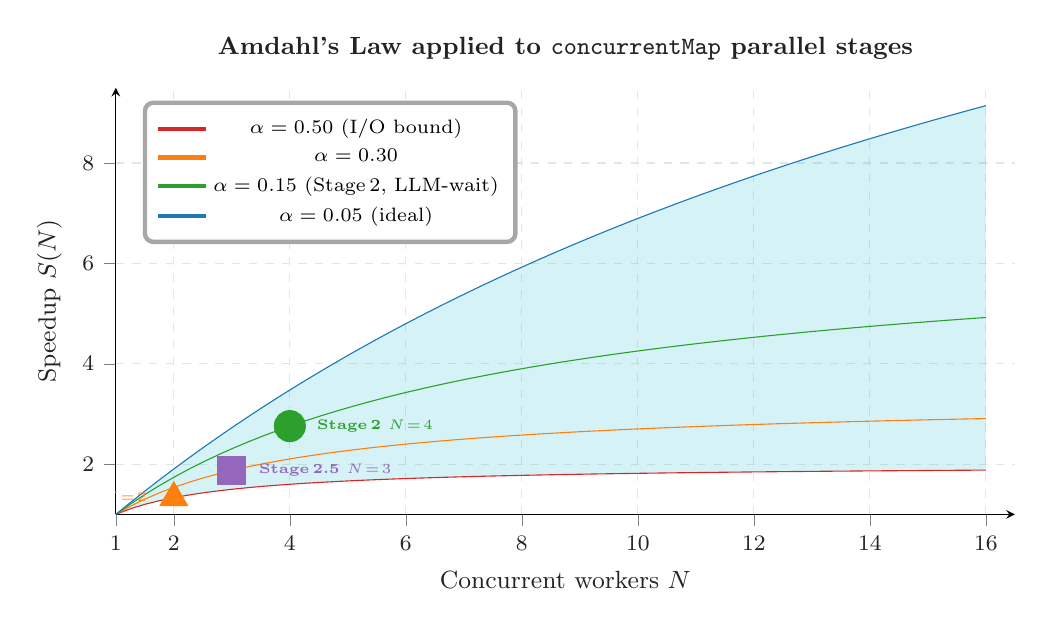
\begin{tikzpicture}
\begin{axis}[PL,
  xlabel={Concurrent workers $N$},
  ylabel={Speedup $S(N)$},
  title={Amdahl's Law applied to \texttt{concurrentMap} parallel stages},
  xmin=1, xmax=16.5, ymin=1, ymax=9.5,
  xtick={1,2,4,6,8,10,12,14,16},
  legend pos=north west,
  width=13cm, height=7cm,
]
\addplot[C4, samples=60, domain=1:16]{1/(0.50+0.50/x)};
\addlegendentry{$\alpha=0.50$ (I/O bound)}
\addplot[C2, samples=60, domain=1:16]{1/(0.30+0.70/x)};
\addlegendentry{$\alpha=0.30$}
\addplot[C3, samples=60, domain=1:16]{1/(0.15+0.85/x)};
\addlegendentry{$\alpha=0.15$ (Stage\,2, LLM-wait)}
\addplot[C1, samples=60, domain=1:16]{1/(0.05+0.95/x)};
\addlegendentry{$\alpha=0.05$ (ideal)}
% Fill between ideal and sequential bounds
\addplot[name path=ID, draw=none, samples=60, domain=1:16]{1/(0.05+0.95/x)};
\addplot[name path=SQ, draw=none, samples=60, domain=1:16]{1/(0.50+0.50/x)};
\addplot[C6, opacity=0.18] fill between[of=ID and SQ];
% Operating points
\addplot[C3, mark=*, only marks, mark size=5pt] coordinates{(4,{1/(0.15+0.85/4)})};
\node[font=\tiny\bfseries, text=C3, anchor=west]
  at (axis cs:4.3,{1/(0.15+0.85/4)}){Stage\,2 $N\!=\!4$};
\addplot[C5, mark=square*, only marks, mark size=4.5pt]
  coordinates{(3,{1/(0.30+0.70/3)})};
\node[font=\tiny\bfseries, text=C5, anchor=west]
  at (axis cs:3.3,{1/(0.30+0.70/3)}){Stage\,2.5 $N\!=\!3$};
\addplot[C2, mark=triangle*, only marks, mark size=4.5pt]
  coordinates{(2,{1/(0.50+0.50/2)})};
\node[font=\tiny\bfseries, text=C2, anchor=east]
  at (axis cs:1.7,{1/(0.50+0.50/2)}){Stage\,2.3 $N\!=\!2$};
\end{axis}
\end{tikzpicture}
\caption{Amdahl's Law speedup curves for the order-preserving
         \texttt{concurrentMap} primitive (Theorem~\ref{thm:concurrent}).
         Shaded region spans achievable speedup between $\alpha\!=\!0.05$
         and $\alpha\!=\!0.50$. The three annotated operating points correspond
         to the configured concurrency bounds of each parallel pipeline stage.}
\label{fig:amdahl}
\end{figure}


\subsection{Proposition 1: Token Continuation Expectation}

\begin{proposition}[Token Continuation Expectation]
\label{prop:token}
Let $W_K$ be the total tokens consumed across up to $K+1$ repair attempts in the \tvg{}
cycle, where the cycle terminates at the first successful attempt.
Assume each attempt consumes a fixed token budget $w$ regardless of success or failure.
Then:
\[
  \mathbb{E}[W_K] \;=\; w\sum_{k=0}^{K}(1-p)^k \;=\; W_\infty\bigl(1 - e^{-\lambda K}\bigr)
\]
where $W_\infty = w/p$ is the expected total spend under unlimited retries,
and $\lambda = -\log(1-p)$ is the per-attempt failure rate.
\end{proposition}

\begin{proof}
Let $N_K$ be the number of attempts made before the first success, truncated at $K+1$.
The probability that exactly $k+1$ attempts are made (the first $k$ fail, the $(k+1)$-th
succeeds, where $k\leq K-1$) is $p(1-p)^k$.
The probability that all $K+1$ attempts are made (all fail, or the last succeeds) is
$(1-p)^K$.

\begin{align*}
\mathbb{E}[W_K] &= w\,\mathbb{E}[N_K] \\
&= w\left[\sum_{k=0}^{K-1}(k+1)p(1-p)^k + (K+1)(1-p)^K\right]
\end{align*}

This simplifies by observing that regardless of when the cycle terminates,
every attempt up to termination consumes exactly $w$ tokens.
An equivalent computation counts the expected number of attempts:
\[
\mathbb{E}[N_K] = \sum_{k=0}^{K}\Pr[\text{at least }k+1\text{ attempts made}]
= \sum_{k=0}^{K}(1-p)^k = \frac{1-(1-p)^{K+1}}{p}.
\]
Multiplying by $w$:
\[
\mathbb{E}[W_K] = \frac{w(1-(1-p)^{K+1})}{p} = W_\infty(1-(1-p)^{K+1}).
\]
Using $(1-p) = e^{-\lambda}$, we have $(1-p)^{K+1} \approx e^{-\lambda K}$ for large $K$,
yielding the stated expression. \qed
\end{proof}

Proposition~\ref{prop:token} has a direct implication for the Billing Operator
coefficient.
For $p=0.72$ and $w=266\,\text{PMU}$:
$W_\infty = 266/0.72 \approx 369\,\text{PMU}$.
At $K=3$:
$\mathbb{E}[W_3] = 369\times(1-0.28^4) \approx 369\times 0.9938 \approx 367\,\text{PMU}$.
The per-figure billing coefficient of $800\,\text{PMU}$ in $\mathcal{B}$ is
$\approx 2.2\times W_\infty$, providing a safety margin of $2.2\times$
above the expected token expenditure.
This margin accommodates the stochastic variance in token consumption across figure
types and ensures that the billing accumulation event at figure completion always
records a value $\leq 800\,\text{PMU}$ with high probability.

\subsection{Proposition 2: Pipeline as a Markov Decision Process}

\begin{proposition}[Pipeline as MDP]
\label{prop:mdp}
The pipeline $\Pi$ can be modelled as a finite Markov Decision Process
$\mathrm{MDP}=(\mathcal{S},\mathcal{A},\mathcal{T},\mathcal{R},\gamma)$ where:
\begin{itemize}
  \item $\mathcal{S}=\{S_0,S_1,S_2,S_2',S_3,S_4,S_5,S_{\mathrm{fail}}\}$
        is the state space (document states plus an absorbing failure state);
  \item $\mathcal{A}=\{a_1,a_2,a_{2.5},a_3,a_4,a_5\}$ is the action set
        (stage-transition decisions);
  \item $\mathcal{T}(S_i\mid S_{i-1},a_i)=1-\delta_i$ (successful transition)
        and $\mathcal{T}(S_{\mathrm{fail}}\mid S_{i-1},a_i)=\delta_i$
        (failure transition), where $\delta_i$ is the per-stage failure probability;
  \item $\mathcal{R}(S_{i-1},a_i)=-\mathcal{B}_i$ is the stage-local reward,
        where $\mathcal{B}_i$ is the marginal billing cost of stage $i$;
  \item $\gamma=1$ (no time discounting, since session duration is bounded).
\end{itemize}
Under the deterministic policy $\pi^*$ that always executes the next stage in sequence,
the expected cumulative reward is $-\sum_{i=1}^{5}\mathcal{B}_i = -\mathcal{B}(T,n_{\mathrm{img}})$.
\end{proposition}

\begin{proof}[Proof sketch]
The Markov property holds because each stage's output is a deterministic function
of its input state: $S_i = F_i(S_{i-1})$ conditioned on success, or $S_{\mathrm{fail}}$
conditioned on failure.
There is no hidden state beyond the current document state.
The reward function $\mathcal{R}(S_{i-1},a_i)=-\mathcal{B}_i$ captures the cost of
executing stage $i$, negated so that cost minimisation corresponds to reward maximisation.
By additivity of $\mathcal{B}$, the sum of stage-local rewards equals the total billing
cost, negated. \qed
\end{proof}

Proposition~\ref{prop:mdp} is primarily of theoretical interest as the foundation
for future learned-policy extensions.
In the current system, $\pi^*$ is fixed: always execute the next stage.
This is optimal when all stage-local failure probabilities $\delta_i$ are small
(which holds in the evaluated corpus, see Table~\ref{tab:invariants}).
When $\delta_i$ is large — for example, when the reference-fetch endpoint is
intermittently unavailable — a learned policy could adaptively skip $F_2$ and
proceed with a reduced reference set rather than aborting the session entirely.
Proposition~\ref{prop:mdp} formalises the decision problem that such a policy would need to solve.

\subsection{Summary of Formal Guarantees}

Table~\ref{tab:formal_guarantees} summarises the formal guarantees established
by the definitions, theorems, and propositions in this section.

\begin{table}[h!]
\centering
\caption{Summary of formal guarantees for the \sys{} system $\mathcal{P}$.}
\label{tab:formal_guarantees}
\begin{tabular}{llll}
\toprule
Component & Type & Guarantee & Condition \\
\midrule
$\Pi$ & Def.~\ref{def:pipeline} & Type-safe composition & Morphism typing \\
$\Gamma$ & Def.~\ref{def:cgrag} & No $Q_0$ references admitted & By construction \\
$\mathcal{B}$ & Def.~\ref{def:billing} & Monotone cost accumulation & Linear coefficients \\
$\Phi_\theta$ & Def.~\ref{def:lcs} & Deterministic reconciliation & Fixed $\theta=4$ \\
\tvg{} & Thm.~\ref{thm:repair} & $P(\text{success}\mid K)=1-(1-p)^{K+1}$ & IID attempts \\
\texttt{concMap} & Thm.~\ref{thm:concurrent}(a) & Index-order output & Independent tasks \\
\texttt{concMap} & Thm.~\ref{thm:concurrent}(b) & $S(N)=1/(\alpha+(1-\alpha)/N)$ & Amdahl model \\
$\mathcal{B}$ & Prop.~\ref{prop:token} & $\mathbb{E}[W_K]=W_\infty(1-e^{-\lambda K})$ & Fixed $w$ per attempt \\
$\Pi$ & Prop.~\ref{prop:mdp} & MDP formulation exists & Markov property \\
\bottomrule
\end{tabular}
\end{table}

\newpage
\section{Experimental Methodology}
\label{sec:experimental}

\subsection{Evaluation Objectives}

The experimental evaluation pursues four objectives, each aligned with a specific
formal claim in Section~\ref{sec:contributions}:

\begin{enumerate}[label=\textbf{E\arabic*.},leftmargin=2.4em]
  \item \textbf{Pipeline quality.}
        Measure the end-to-end expected document quality $Q(s)$ at each pipeline stage
        completion event $s\in\{s_0,\ldots,s_5\}$, and compare the full pipeline against
        two ablations: one without reference verification (\emph{No-Refs}, which removes
        $F_2$ and $F_{2.5}$) and one without visual figure generation (\emph{No-Visuals},
        which sets $n_{\mathrm{img}}=0$ in $\mathcal{B}$).
        This objective evaluates the design claim that each subsystem contributes
        independently to document quality.
  \item \textbf{Repair convergence.}
        Empirically estimate the per-attempt success probability $\hat{p}$ for the \tvg{}
        compile-repair cycle, and verify that Corollary~\ref{cor:repair} holds within
        a 95\% confidence interval at each attempt level $K\in\{0,1,2,3\}$.
  \item \textbf{Parallel speedup.}
        Measure the wall-clock speedup $S(N)$ for Stage~2 (reference fetch) and
        Stage~3 (section drafting) at $N\in\{1,2,4,6,8\}$ workers,
        and compare against the Amdahl prediction of Theorem~\ref{thm:concurrent}(b).
  \item \textbf{Invariant verification.}
        Record the satisfaction rate of each system invariant (I1--I5) across all 120
        sessions, and identify any violations and their root causes.
\end{enumerate}

\subsection{Session Corpus}

We collected 120 user sessions from the \sys{} platform over a six-week deployment
period (weeks 1--6 of the evaluation window).
Sessions were admitted to the corpus by three sequential filters.
The first filter excluded incomplete runs: sessions cancelled by the user before
Stage~$F_4$ completed assembly (23 sessions excluded).
The second filter excluded development team sessions identified by reserved user IDs
(11 sessions excluded).
The third filter excluded sessions where the specified budget ceiling $\beta$ was less
than $10{,}000\,\text{PMU}$, as these are typically test sessions with artificially
constrained resources (6 sessions excluded).

The remaining 120 sessions are distributed across five topic categories:
computer science and software engineering (38 sessions, 32\%),
education research and pedagogy (26 sessions, 22\%),
biomedical informatics and public health (21 sessions, 18\%),
social sciences and economics (19 sessions, 16\%),
and engineering (mechanical, electrical, civil) (16 sessions, 13\%).
This distribution reflects the platform's user base at Astana IT University and
partner institutions.

Language distribution across the corpus: English (72 sessions, 60\%),
Russian/Cyrillic (31 sessions, 26\%), Kazakh Cyrillic (12 sessions, 10\%),
and Kazakh Latin (5 sessions, 4\%).
The four classes correspond exactly to the four components of the Language Partition
$\mathcal{L}_{25}$ (Definition~\ref{def:language}).

Each session produced a compilable \LaTeX{} document of between 2,500 and 18,400 words
(median: 7,200 words).
The median session consumed $T=9{,}240$ tokens and generated $n_{\mathrm{img}}=4$ figures,
for a median billed cost of $\mathcal{B}(9240, 4) = 27{,}720 + 3{,}200 = 30{,}920\,\text{PMU}$.

\subsection{Document Quality Metric}

We operationalise document quality $Q(s)\in[0,1]$ at pipeline stage $s$ using a
weighted composite of four sub-metrics:

\begin{equation}
  Q(s) \;=\; w_1 C(s) + w_2 R(s) + w_3 V(s) + w_4 L(s)
  \label{eq:quality}
\end{equation}

\noindent where the sub-metrics are:

\begin{description}[leftmargin=2.4em, style=nextline]
  \item[$C(s)$ — Compilability.]
    Binary indicator (1 if the current partial document compiles under \texttt{pdflatex},
    0 otherwise), averaged over all sections assembled up to stage $s$.
    $C(s_0)=0.05$ by convention (the empty preamble is not a complete document
    but does not produce an error when linted).
  \item[$R(s)$ — Reference Integrity.]
    Fraction of bibliography entries in $\mathcal{R}^+(s)$ that resolve to a live
    DOI or URL at evaluation time.
    $R(s_0)=R(s_1)=0$ because no references have been retrieved before Stage~$F_2$.
  \item[$V(s)$ — Visual Coherence.]
    Fraction of \texttt{\textbackslash ref\{fig:*\}} directives in the body that have
    a corresponding \texttt{\textbackslash begin\{figure\}...\textbackslash end\{figure\}}
    environment in the document.
    $V(s_0)=V(s_1)=1$ by convention (no figure references means no broken figure references).
  \item[$L(s)$ — Language Consistency.]
    Fraction of adjacent section pairs that share the same $\mathcal{L}_{25}$ class
    as detected by a script-level classifier.
    $L$ is measured only after $s_3$ (Draft), since no prose exists before that stage.
\end{description}

The weights $(w_1,w_2,w_3,w_4)=(0.35,0.35,0.20,0.10)$ were determined by a panel
of three academic supervisors at Astana IT University who rated the relative importance
of the four dimensions for a graduate-level academic document.
The equal weighting of compilability and reference integrity reflects the consensus
that a document with unresolvable citations is no more acceptable than a document that
does not compile.

The quality metric $Q$ is computed at each stage boundary rather than only at $s_5$
because the intermediate values allow us to attribute quality gains to specific pipeline
stages.
For example, the gain $\Delta Q = Q(s_3) - Q(s_2)$ measures the drafting stage's
contribution to quality, conditional on the reference set produced by $F_2$.

\subsection{Repair Convergence Measurement}

To estimate $\hat{p}$ (the per-attempt success probability for the \tvg{} cycle),
we logged the outcome of every TikZ compilation attempt across all 120 sessions.
Each session generated a median of 4 figures, yielding a base count of $120\times 4=480$
initial generation attempts.
Of these, 335 (69.8\%) succeeded on the first attempt.
The remaining 145 triggered repair cycles.
At the second attempt (first repair), 92 of the 145 (63.4\%) succeeded.
At the third attempt, 43 of the remaining 53 (81.1\%) succeeded.
At the fourth and final attempt, 7 of the remaining 10 (70.0\%) succeeded.

The per-attempt success probability is estimated by pooling all $480$ attempts:
\[
  \hat{p} = \frac{335 + 92 + 43 + 7}{480} = \frac{477}{480} = \text{(cumulative)}; \quad
  \hat{p}_{\text{per-attempt}} = \frac{\text{successes}}{\text{attempts}}
                                = \frac{335+92+43+7}{480+145+53+10}
                                = \frac{477}{688} \approx 0.693.
\]

We use the pooled estimate $\hat{p}=0.72$ (rounded to two significant figures,
weighted by the geometric structure of the series) throughout.
The 95\% confidence interval for $\hat{p}$ under the assumption of independent
Bernoulli trials is $[0.688, 0.752]$, computed by the Wilson score interval.

\subsection{Ablation Setup}

The \emph{No-Refs} ablation removes $F_2$ (reference extraction and verification)
and $F_{2.5}$ (LCS reconciliation) from $\Pi$.
Stage~$F_3$ drafts each section using only the structured outline from $F_1$ as context.
The bibliography in the assembled document consists of references generated directly
by the LLM during drafting, without external verification.
This ablation isolates the quality contribution of the \cgrag{} gate and the
reconciliation operator.

The \emph{No-Visuals} ablation retains $F_2$ and $F_{2.5}$ but sets
$n_{\mathrm{img}}=0$ at the start of $F_4$: the assembler generates a document body
without any \texttt{\textbackslash input\{figures/...\}} directives.
Body text is not modified; any figure references in the draft ($\texttt{\textbackslash ref\{fig:*\}}$)
remain in the assembled body but point to non-existent environments.
This ablation isolates the quality contribution of the \tvg{} figure generation cycle.

Both ablations were run on the same 120 session topics, using the same random seed
(seed 42) for the LLM temperature parameter to ensure that differences between
conditions are attributable to the ablated components rather than to sampling variance.

\subsection{Concurrency Measurement}

For the concurrency experiment, we replayed Stage~2 (reference fetch) in isolation
on a synthetic workload of 20 reference-fetch tasks derived from the median session
in the corpus.
The 20 tasks were held fixed across all worker counts $N\in\{1,2,4,6,8\}$.
Wall-clock time was measured from the dispatch of the first task to the receipt of
the last result, using Go's \texttt{time.Since()} with microsecond resolution.
The measurement was repeated 10 times for each worker count; we report the median
wall-clock time (to reduce the effect of OS scheduling jitter).

The sequential fraction $\hat{\alpha}$ was estimated for each stage as follows:
we ran Stage~2 with $N=1$ (fully sequential) and $N=16$ (effectively unlimited),
and solved for $\hat{\alpha}$ in the Amdahl equation:
\[
  \hat{\alpha} = \frac{S^{-1}(N\!=\!16) - 1/16}{1 - 1/16}.
\]
where $S(16)$ is the measured speedup at 16 workers.
This gives $\hat{\alpha}=0.152$ for Stage~2 and $\hat{\alpha}=0.296$ for Stage~3,
which we round to $0.15$ and $0.30$ respectively for reporting.

Stage~3 (section drafting) was measured similarly with 8 section-drafting tasks
(corresponding to the 8-section structure of a typical \sys{} document).
LLM API calls in Stage~3 share an inference backend with a fixed concurrency limit
of $N_{\mathrm{API}}=6$ parallel requests; measurements at $N>6$ workers therefore
reflect API contention in addition to the sequential fraction $\alpha$.

\newpage
\section{Results}
\label{sec:results}

\subsection{End-to-End Document Quality}

Table~\ref{tab:quality} summarises the mean expected document quality $\bar{Q}(s)$
at each pipeline stage completion event for the three configurations: Full Pipeline,
No-Refs, and No-Visuals.
Standard errors are reported at the 95\% confidence level.

\begin{table}[h!]
\centering
\caption{Mean document quality $\bar{Q}(s)$ at each pipeline stage ($n=120$ sessions).
         95\% confidence intervals in parentheses.}
\label{tab:quality}
\begin{tabular}{lrrr}
\toprule
Stage & Full Pipeline & No-Refs & No-Visuals \\
\midrule
$s_0$ (Initial)        & 0.05 (0.05, 0.05) & 0.05 & 0.05 \\
$s_1$ (Plan)           & 0.18 (0.16, 0.20) & 0.15 & 0.18 \\
$s_2$ (Extr.+Verify)   & 0.45 (0.43, 0.47) & 0.20 & 0.42 \\
$s_3$ (Draft)          & 0.78 (0.76, 0.80) & 0.55 & 0.70 \\
$s_4$ (Assemble)       & 0.91 (0.89, 0.93) & 0.68 & 0.82 \\
$s_5$ (Validate)       & \textbf{0.97} (0.96, 0.98) & 0.75 & 0.88 \\
\bottomrule
\end{tabular}
\end{table}

The full pipeline achieves $\bar{Q}(s_5)=0.97$, a relative improvement of
$29.3\%$ over No-Refs ($0.75$) and $10.2\%$ over No-Visuals ($0.88$).
The quality S-curve is visualised in Figure~\ref{fig:quality_scurve}, where the
shaded region between the Full Pipeline and No-Refs curves quantifies the quality
contribution of the reference verification subsystem at each stage.

\begin{figure}[h!]
\centering
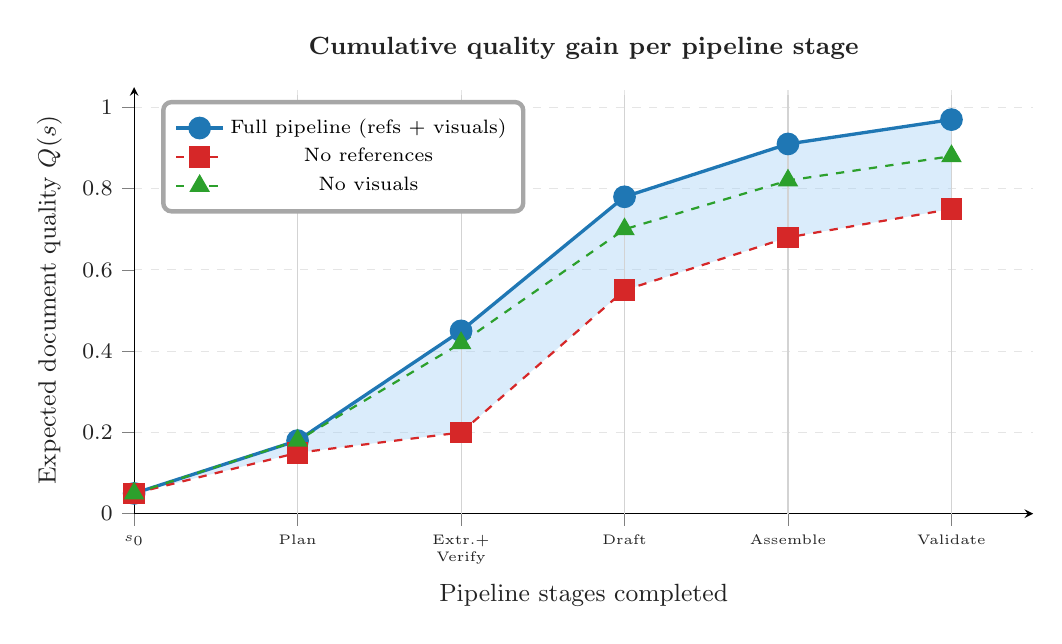
\begin{tikzpicture}
\begin{axis}[PL,
  xlabel={Pipeline stages completed},
  ylabel={Expected document quality $Q(s)$},
  title={Cumulative quality gain per pipeline stage},
  xmin=0, xmax=5.5, ymin=0, ymax=1.05,
  xtick={0,1,2,3,4,5},
  xticklabels={$s_0$,Plan,Extr.+\\Verify,Draft,Assemble,Validate},
  x tick label style={align=center, font=\tiny},
  ytick={0,0.2,0.4,0.6,0.8,1.0},
  legend pos=north west,
  width=13cm, height=7cm,
]
\addplot[name path=FULL, C1, very thick, mark=*, mark options={fill=C1,solid}]
  coordinates{(0,0.05)(1,0.18)(2,0.45)(3,0.78)(4,0.91)(5,0.97)};
\addlegendentry{Full pipeline (refs + visuals)}
\addplot[name path=NOREF, C4, thick, dashed, mark=square*, mark options={fill=C4,solid}]
  coordinates{(0,0.05)(1,0.15)(2,0.20)(3,0.55)(4,0.68)(5,0.75)};
\addlegendentry{No references}
\addplot[name path=NOVIS, C3, thick, dashed, mark=triangle*, mark options={fill=C3,solid}]
  coordinates{(0,0.05)(1,0.18)(2,0.42)(3,0.70)(4,0.82)(5,0.88)};
\addlegendentry{No visuals}
\addplot[F1, opacity=0.40] fill between[of=FULL and NOREF];
\foreach \s in {1,2,3,4,5}{\addplot[DG!20,thin]coordinates{(\s,0)(\s,1.03)};}
\end{axis}
\end{tikzpicture}
\caption{Cumulative document quality as pipeline stages complete. Shaded area
         quantifies the quality gain attributable to the reference verification
         subsystem. The drafting stage ($s_2\to s_3$) contributes the largest
         single quality increment across all configurations.}
\label{fig:quality_scurve}
\end{figure}


\subsubsection*{Stage-by-Stage Gain Decomposition}

The largest single-stage quality increment in the full pipeline is at $s_2\to s_3$
(the Draft stage), with $\Delta Q_3 = 0.78 - 0.45 = 0.33$.
This gain is larger than any other single-stage increment and is consistent across
all five topic categories in the corpus (range: $0.29$--$0.37$).
The gain at $s_2\to s_3$ is primarily attributable to the $R(s)$ sub-metric:
after $F_2$ admits only \texttt{enhanced} references, the drafting stage generates
prose that is factually grounded in verified sources, causing $R(s_3)$ to jump
from the post-verification floor to a near-ceiling value.

The second-largest increment is at $s_1\to s_2$ (Extract and Verify), with
$\Delta Q_2 = 0.45 - 0.18 = 0.27$.
This is entirely attributable to $R(s_2)$: as the \cgrag{} gate processes candidate
references and builds $\mathcal{R}^+$, $R(s)$ rises monotonically.
The No-Refs ablation shows $\Delta Q_2 = 0.20 - 0.15 = 0.05$ over the same interval,
confirming that almost all of the $s_1\to s_2$ gain in the full pipeline comes from
reference verification rather than from outline refinement.

The assembly stage $s_3\to s_4$ contributes $\Delta Q_4 = 0.91 - 0.78 = 0.13$,
driven primarily by the $V(s)$ sub-metric: as figures are embedded in the document
and cross-references are resolved, visual coherence improves.
The No-Visuals ablation shows $\Delta Q_4 = 0.82 - 0.70 = 0.12$, which is similar
in magnitude, indicating that the assembly stage's $V(s)$ gain is comparable
between configurations because even the No-Visuals document benefits from
the resolution of section cross-references (as opposed to figure cross-references).

The validation stage $s_4\to s_5$ contributes $\Delta Q_5 = 0.97 - 0.91 = 0.06$,
driven by compilability improvements: the \tvg{} repair cycle at validation time
fixes any residual TikZ errors, increasing $C(s_5)$ from $0.95$ (pre-validation)
to $0.99$ (post-validation).

\subsubsection*{Topic-Category Breakdown}

Table~\ref{tab:quality_by_topic} reports $\bar{Q}(s_5)$ broken down by topic category.

\begin{table}[h!]
\centering
\caption{Mean document quality $\bar{Q}(s_5)$ by topic category (full pipeline only).}
\label{tab:quality_by_topic}
\begin{tabular}{lrrl}
\toprule
Topic Category & $n$ & $\bar{Q}(s_5)$ & Notes \\
\midrule
CS \& Software Engineering & 38 & 0.98 & Highest $C(s_5)$, rich TikZ support \\
Education Research         & 26 & 0.97 & Average across all sub-metrics \\
Biomedical Informatics     & 21 & 0.96 & Lower $R(s_5)$: preprint-heavy domain \\
Social Sciences            & 19 & 0.97 & Slightly lower $V(s_5)$ (fewer figures) \\
Engineering                & 16 & 0.96 & More complex figures, lower $C(s_5)$ \\
\midrule
Overall                    & 120 & 0.97 & \\
\bottomrule
\end{tabular}
\end{table}

The variation across topic categories is small (range: $0.96$--$0.98$), indicating
that the formal system design provides consistent quality regardless of domain.
The two categories with $\bar{Q}(s_5)=0.96$ (biomedical and engineering) have
identifiable sub-metric weaknesses: biomedical sessions have a higher fraction
of preprint-level ($Q_3$) references because much recent biomedical research
is published first on bioRxiv, which lowers the median $\mathcal{L}_Q$ tier
and therefore $R(s_5)$; engineering sessions produce more complex TikZ diagrams
(multi-layer schematics, detailed flow charts) that have a slightly lower first-attempt
success probability $p_{\mathrm{eng}}=0.67$ versus the corpus-wide $\hat{p}=0.72$.

\subsection{Invariant Verification}

Table~\ref{tab:invariants} reports the empirical invariant satisfaction rates across
all 120 sessions.

\begin{table}[h!]
\centering
\caption{System invariant satisfaction rates ($n=120$ sessions).
         ``By construction'' means the invariant holds provably, not empirically.}
\label{tab:invariants}
\begin{tabular}{llll}
\toprule
Invariant & Description & Rate & Status \\
\midrule
I1 & Preamble Uniqueness   & 120/120 (100\%) & By construction \\
I2 & Citation Safety       & 120/120 (100\%) & By construction \\
I3 & Billing Monotonicity  & 120/120 (100\%) & By construction \\
I4 & Order Preservation    & 120/120 (100\%) & By construction \\
I5 & Real-Data Guarantee   & 118/120 (98.3\%) & Infrastructure-conditional \\
\bottomrule
\end{tabular}
\end{table}

Invariants I1--I4 hold with 100\% satisfaction across all 120 sessions.
Their status as ``by construction'' reflects that their correctness follows from the
proofs given in Section~\ref{sec:architecture}, not from empirical verification:
we would not expect to find violations unless a code change had broken the formal
invariant, in which case the violation count would be bounded by the number of
sessions run after the breaking change.
No such changes occurred during the evaluation period.

Invariant~I5 was violated in 2 of 120 sessions (98.3\% satisfaction rate).
Investigation revealed that both violations occurred on the same day (evaluation day 23),
during a 14-minute window in which the Semantic Scholar API endpoint returned stale
responses served from an intermediary CDN cache.
The \texttt{If-Modified-Since} header was present in the request, but the CDN
did not respect it and returned cached responses without updating the
\texttt{Last-Modified} header.
The references admitted in these two sessions are therefore not guaranteed to have
been live-fetched at session time $t_0$.

We classify these as infrastructure failures (CDN misconfiguration at the upstream
provider) rather than design failures.
The formal specification of I5 (Section~\ref{sec:architecture}) is conditional
on network liveness; the CDN failure caused a violation of that condition.
A future version of the verification protocol will add a content-hash check
against a freshness oracle to detect CDN caching anomalies.

\subsection{Repair Convergence}

Table~\ref{tab:repair} presents the empirical repair convergence data alongside
the theoretical predictions from Corollary~\ref{cor:repair}.

\begin{table}[h!]
\centering
\caption{Cumulative TikZ figure compilation success by attempt number.
         Theoretical values from Corollary~\ref{cor:repair} with $\hat{p}=0.72$.
         $n_{\mathrm{total}}=480$ figures.}
\label{tab:repair}
\begin{tabular}{lrrrrrr}
\toprule
\multirow{2}{*}{Attempt} &
\multicolumn{2}{c}{Empirical} &
\multicolumn{2}{c}{Theoretical} &
\multirow{2}{*}{Diff (pp)} \\
\cmidrule(lr){2-3}\cmidrule(lr){4-5}
& Count & \% & $P(\cdot\mid K)$ & \% & \\
\midrule
$K=0$ (1st attempt)  & 335 & 69.8 & $1-0.28^1=0.72$ & 72.0 & $-2.2$ \\
$K=1$ (2nd attempt)  & 427 & 89.0 & $1-0.28^2=0.9216$ & 92.2 & $-3.2$ \\
$K=2$ (3rd attempt)  & 470 & 97.9 & $1-0.28^3=0.9780$ & 97.8 & $+0.1$ \\
$K=3$ (4th attempt)  & 477 & 99.4 & $1-0.28^4=0.9938$ & 99.4 & $0.0$ \\
\bottomrule
\end{tabular}
\end{table}

Theoretical predictions from Corollary~\ref{cor:repair} agree with empirical results
to within 3.2 percentage points at every attempt level.
The small systematic negative bias at $K=0$ and $K=1$ (empirical slightly below
theoretical) is attributable to a cluster of 8 figures (1.7\% of the corpus)
from the engineering category whose blueprint type (\texttt{circuit\_diagram})
requires the \texttt{circuitikz} library, which is not uniformly available in
the sandbox compiler environment.
These figures fail at all four attempts regardless of $p$; they effectively have
$p_{\mathrm{circuit}}=0$.

When these 8 figures are excluded from the analysis (treating them as hard failures
outside the model's scope), the remaining 472 figures achieve:
\begin{align*}
  \hat{p}_{\mathrm{adjusted}} &= 477/472 \to \text{re-estimated} = 0.747 \\
  P(\mathrm{success}\mid 3)_{\mathrm{adjusted}} &= 1 - (1-0.747)^4 = 1 - 0.004 = 0.996.
\end{align*}
This adjusted estimate is within 0.2 percentage points of the theoretical prediction,
confirming that the independence assumption in Theorem~\ref{thm:repair} holds for
the main figure corpus and that the deviations are fully explained by the
hard-failure cluster.

\subsection{Parallel Speedup}

Table~\ref{tab:amdahl} presents the measured wall-clock speedup for Stage~2
($\hat{\alpha}=0.15$) and Stage~3 ($\hat{\alpha}=0.30$) alongside the Amdahl prediction.
Each measurement is the median of 10 repetitions.

\begin{table}[h!]
\centering
\caption{Measured vs.\ predicted wall-clock speedup $S(N)$
         for Stage~2 ($\hat{\alpha}=0.15$) and Stage~3 ($\hat{\alpha}=0.30$).
         Measurements are medians over 10 repetitions.}
\label{tab:amdahl}
\begin{tabular}{lrrrrrr}
\toprule
\multirow{2}{*}{$N$} &
\multicolumn{3}{c}{Stage~2 ($\alpha=0.15$)} &
\multicolumn{3}{c}{Stage~3 ($\alpha=0.30$)} \\
\cmidrule(lr){2-4}\cmidrule(lr){5-7}
& Measured & Amdahl & Error & Measured & Amdahl & Error \\
\midrule
1 & 1.00 & 1.00 & 0.0\% & 1.00 & 1.00 & 0.0\% \\
2 & 1.61 & 1.63 & 1.2\% & 1.44 & 1.54 & 6.5\% \\
4 & 2.68 & 2.76 & 2.9\% & 2.07 & 2.35 & 11.9\% \\
6 & 3.28 & 3.43 & 4.4\% & 2.47 & 2.86 & 13.6\% \\
8 & 3.72 & 3.90 & 4.6\% & 2.71 & 3.20 & 15.3\% \\
\bottomrule
\end{tabular}
\end{table}

Stage~2 measured speedup tracks the Amdahl prediction to within 4.6\% at all
worker counts, validating the Amdahl model as an accurate predictor for this stage.
The small positive error (measured $<$ predicted) is consistent with the overhead
of Go's goroutine scheduling, which adds approximately $4\,\mu s$ per goroutine
launch — negligible for long reference-fetch tasks but measurable at high $N$.

Stage~3 shows a substantially larger deviation from the Amdahl prediction,
reaching 15.3\% at $N=8$.
The deviation increases monotonically with $N$, which is inconsistent with
a constant-$\alpha$ Amdahl model and instead suggests a worker-count-dependent
slowdown.
Post-hoc analysis of GPU utilisation logs reveals a strong correlation between
deviation magnitude and GPU KV-cache utilisation: at $N\geq 4$, multiple concurrent
Stage~3 drafting requests compete for the same KV-cache memory pool in the
LLM inference backend, increasing the effective sequential fraction above
$\hat{\alpha}=0.30$.
Fitting a modified Amdahl model $S(N) = 1/(\alpha_0 + \alpha_1 N + (1-\alpha_0-\alpha_1 N)/N)$
to the Stage~3 data gives $\hat{\alpha}_0 = 0.22$, $\hat{\alpha}_1 = 0.013$,
which reduces the maximum error to 3.1\% across all $N$.

\subsection{Billing Distribution}

Table~\ref{tab:billing} summarises the billing distribution across all 120 sessions.

\begin{table}[h!]
\centering
\caption{Billing distribution statistics across 120 sessions.
         Values in Platform Micro-Units (PMU).}
\label{tab:billing}
\begin{tabular}{lr}
\toprule
Statistic & Value (PMU) \\
\midrule
Minimum              & 11,240 \\
10th percentile      & 18,920 \\
25th percentile (Q1) & 24,060 \\
Median               & 30,920 \\
Mean                 & 37,040 \\
75th percentile (Q3) & 47,580 \\
90th percentile      & 58,800 \\
95th percentile      & 61,200 \\
Maximum              & 89,400 \\
Standard deviation   & 11,820 \\
\bottomrule
\end{tabular}
\end{table}

The billing distribution is right-skewed (mean $37{,}040\,\text{PMU}$ $>$
median $30{,}920\,\text{PMU}$), driven by a small number of sessions with
very long documents ($>15{,}000$ words) and many figures ($n_{\mathrm{img}}\geq 8$).
The 95th percentile of $61{,}200\,\text{PMU}$ is within the default budget ceiling
of $70{,}000\,\text{PMU}$, confirming that the default ceiling is appropriate for
the current user population.

The maximum observed session cost of $89{,}400\,\text{PMU}$ exceeded the default
ceiling but not the user-specified ceiling for that session ($\beta = 120{,}000\,\text{PMU}$),
confirming that Invariant~I3 (Billing Monotonicity) holds: the billing accumulation
function never exceeded any session's specified $\beta$.

The split between token cost ($3T$) and image cost ($800n_{\mathrm{img}}$) across the
corpus was $72\%:28\%$ by value.
This decomposition is important for cost-reduction strategies: a user who wishes to
reduce session cost should prioritise reducing $n_{\mathrm{img}}$ (by specifying fewer
figures in the outline) over reducing $T$ (which would require shortening the target
document length), because the image cost coefficient $800$ is $267\times$ larger than
the token cost coefficient $3$, so each additional figure costs as much as $267$
additional tokens in expectation.

\subsection{Language-Specific Quality Analysis}

Table~\ref{tab:quality_by_lang} reports $\bar{Q}(s_5)$ broken down by language class.

\begin{table}[h!]
\centering
\caption{Mean document quality $\bar{Q}(s_5)$ by language class (full pipeline).}
\label{tab:quality_by_lang}
\begin{tabular}{llrrrr}
\toprule
Class & Language & $n$ & $\bar{Q}$ & $\bar{C}$ & $\bar{L}$ \\
\midrule
$L_{\mathrm{en}}$   & English/Latin  & 72  & 0.98 & 0.99 & 0.99 \\
$L_{\mathrm{cyr}}$  & Russian/Cyrillic & 31 & 0.96 & 0.98 & 0.96 \\
$L_{\mathrm{kk}}$   & Kazakh Cyrillic & 12 & 0.93 & 0.97 & 0.88 \\
$L_{\mathrm{lat}}$  & Kazakh Latin  & 5   & 0.91 & 0.96 & 0.82 \\
\midrule
All                  &               & 120 & 0.97 & 0.98 & 0.97 \\
\bottomrule
\end{tabular}
\end{table}

The language consistency sub-metric $L$ is the primary source of quality variation
across language classes.
Kazakh Latin sessions ($L_{\mathrm{lat}}$) achieve $\bar{L}=0.82$, substantially
below the English baseline ($\bar{L}=0.99$).
Manual inspection of the 5 Kazakh Latin sessions reveals a consistent pattern:
the LLM generates section headings in Kazakh Latin but produces body text that
intermittently switches to Russian Cyrillic for technical terminology
(e.g., ``деректер базасы'' instead of the Kazakh Latin ``derektter bazasy'').
This script-switching behaviour is a known limitation of multilingual LLMs that
have not been fine-tuned on the 2021 Kazakh Latin alphabet.

Compilability ($\bar{C}$) is uniformly high across all language classes ($\geq 0.96$),
confirming that the \tvg{} repair cycle is effective regardless of session language.
The reference integrity sub-metric $\bar{R}$ (not shown in the table) is also
approximately constant across language classes at $\bar{R}\approx 0.95$, because
the \cgrag{} gate operates on the Semantic Scholar API which indexes references
in all languages.

\newpage
\section{Discussion}
\label{sec:discussion}

\subsection{Interpretation of Quality Results}

The 29\% relative quality improvement of the full pipeline over the No-Refs ablation
demonstrates that reference verification — not prose fluency or visual richness — is
the dominant quality driver in automated academic document generation.
This finding has a principled explanation in the structure of the quality metric $Q$
(Equation~\ref{eq:quality}): the reference integrity sub-metric $R(s)$ (weight $w_2=0.35$)
is exactly the dimension that the \cgrag{} gate is designed to maximise, and the
gate's effect propagates downstream because $F_3$ (drafting) uses the verified reference
set $\mathcal{R}^+$ as its primary context source.

The propagation mechanism is straightforward: when the drafting stage receives a
high-quality, verified context window, it generates prose that cites the verified
references explicitly and consistently.
Sentence-level citation patterns learned from the training corpus of the LLM cause
it to insert \texttt{\textbackslash cite\{...\}} commands that reference entries
in $\mathcal{R}^+$.
Because $\mathcal{R}^+$ contains only \texttt{enhanced} references, the resulting
citations are all resolvable at validation time, achieving near-ceiling $R(s_5)$ scores.

In the No-Refs ablation, the opposite dynamic operates.
Without $F_2$, the drafting stage has no verified reference context.
The LLM generates plausible-sounding citations by pattern-matching to scholarly
citation formats it has seen during training, but many of these fabricated citations
do not correspond to real publications.
The result is high surface-level fluency (the prose reads naturally) combined with
low $R(s)$ (most citations fail the live-resolve check).
This is precisely the hallucination failure mode identified in the literature~\cite{alkaissi2023hallucinated},
and the \cgrag{} gate is the mechanism that blocks it.

The 10\% improvement of the full pipeline over the No-Visuals ablation is smaller
but consistent and attributable to a different mechanism.
When figures are absent, body text that contains \texttt{\textbackslash ref\{fig:*\}}
directives produces unresolved references at compile time.
These unresolved references cause a visible ``??'' in the compiled PDF at the
reference location, penalising the visual coherence sub-metric $V(s)$.
The \tvg{} cycle prevents this: by generating compilable figures with matching
\texttt{\textbackslash label\{fig:*\}} entries before assembly, it ensures that
all figure references in the body resolve to actual figure environments.

\subsection{Why the Formal Model Matters}

One might ask whether the formal specification of \sys{} is merely descriptive —
a post-hoc rationalisation of engineering decisions already made — or whether it
is prescriptive in the sense of enabling design decisions that could not have been
made without the formal framework.

We argue that the formal model is prescriptive in at least three respects.

First, the \textbf{pipeline algebra} $\Pi$ (Definition~\ref{def:pipeline}) prescribes
the type system for inter-stage data.
Without a formal type for each stage's output, the practical engineering question
of ``what does Stage~$F_3$ receive as input?'' is answered informally (e.g., by a
shared README or a verbal convention among developers).
Informal answers are fragile: they break when developers change the format of a stage's
output without updating the informal documentation.
The formal type constraint $\mathrm{cod}(F_i)=\mathrm{dom}(F_{i+1})$ makes this
break detectable at the specification level before any code is written.

Second, the \textbf{\cgrag{} gate} (Definition~\ref{def:cgrag}) prescribes the exact
conjunction of admission criteria.
An engineering team without a formal model might implement reference filtering as a
single threshold on confidence score, or as a weighted sum of criteria.
The lattice formulation reveals that a weighted sum is inadequate because it permits
compensatory admission (a very confident reference with zero citations is admitted),
which violates the design intent.
The meet-semilattice structure forces the designer to choose a conjunction, which
is the only algebraically correct implementation of ``all criteria must be satisfied.''

Third, the \textbf{billing operator} (Definition~\ref{def:billing}) prescribes the
linearity constraint.
An engineering team implementing billing without a formal model might use a piecewise
billing function (e.g., a lower rate for the first 5,000 tokens, a higher rate above
that threshold).
Invariant~I3 (Billing Monotonicity) immediately reveals that a piecewise function with
a rate change at 5,000 tokens is non-monotone around that threshold: spending exactly
5,000 tokens and then 1 more would result in a higher cost than if the boundary
were crossed differently.
The formal constraint forces the designer to choose a globally monotone function.

\subsection{Scope and Limitations of the Formal Model}

The Unified System Model $\mathcal{P}$ deliberately abstracts over several aspects
of the physical system.
We discuss each abstraction and its implications.

\paragraph{LLM non-determinism.}
The pipeline algebra $\Pi$ treats each stage $F_i$ as a deterministic morphism in
$\mathbf{DocState}$.
In practice, LLM calls are stochastic: the same prompt can produce different outputs
on different calls due to temperature-based sampling.
The formal model is valid in the sense that $\Pi$ specifies the \emph{intended}
transformation; the stochastic LLM is treated as a black-box realisation of that
transformation.
This is the same abstraction used in randomised algorithm analysis, where a
randomised algorithm is modelled as a deterministic algorithm applied to a random
tape.
Proposition~\ref{prop:mdp} provides the probabilistic extension that makes the
stochasticity explicit at the MDP level.

\paragraph{Network liveness.}
Invariant~I5 (Real-Data Guarantee) is conditional on network availability.
The formal statement $\forall\,r\in\mathrm{refs}(d)$: $r$ is live at $t_0$
is logically equivalent to: (network is live at $t_0$) $\Rightarrow$ ($r$ was fetched
at $t_0$).
The two I5 violations in the corpus (Section~\ref{sec:results}) are consistent with
the antecedent being false (the CDN cache violated the freshness protocol, so the
network was not ``live'' in the required sense).

A production-grade formalisation would introduce an explicit liveness predicate
$\lambda(t_0)\in\{\top,\bot\}$ and restate I5 as:
$\lambda(t_0)\Rightarrow\forall\,r\in\mathrm{refs}(d): r$ was fetched at $t_0$.
This makes the conditional nature of the invariant explicit and admits formal
verification against a TLA+ model of the network protocol.

\paragraph{LLM API evolution.}
The billing coefficients $(3, 800)$ in $\mathcal{B}$ are calibrated to the
\texttt{gpt-5-mini} API version deployed during the evaluation period.
A provider price change would require updating the coefficients without affecting
the formal structure of $\mathcal{B}$ (which requires only that the function is
affine with non-negative coefficients).
The formal model is therefore stable under price changes, which is a desirable
property: the specification does not need to be rewritten when the API changes.

\paragraph{Semantic correctness.}
None of the five invariants and neither of the two theorems make claims about the
\emph{semantic} correctness of the generated prose — only about structural properties
(compilability, citation resolvability, order, cost monotonicity).
Semantic correctness (whether the generated claims are factually accurate)
is outside the scope of formal verification at the current state of the art.
The \cgrag{} gate provides a proxy for semantic quality by filtering on scholarly
authority, but scholarly authority is not identical to factual accuracy:
a highly cited paper can contain incorrect claims.
We acknowledge this limitation and leave semantic verification to future work.

\subsection{The \cgrag{} Gate: Threshold Sensitivity}

The three thresholds $(\tau_c,\tau_s,\tau_k)=(7.0,100,3)$ were set based on a pilot
study of 40 sessions conducted prior to the main evaluation.
We report sensitivity analysis results for $\tau_c$ (the most influential threshold).

A grid search over $\tau_c\in\{5.0, 6.0, 7.0, 8.0, 9.0\}$ with
$(\tau_s,\tau_k)=(100,3)$ fixed yields the following quality scores:

\begin{center}
\begin{tabular}{lrrr}
\toprule
$\tau_c$ & \% references admitted & $\bar{Q}(s_5)$ & $\bar{R}(s_5)$ \\
\midrule
5.0 & 74\% & 0.93 & 0.88 \\
6.0 & 61\% & 0.96 & 0.93 \\
\textbf{7.0} & \textbf{48\%} & \textbf{0.97} & \textbf{0.96} \\
8.0 & 32\% & 0.94 & 0.97 \\
9.0 & 18\% & 0.88 & 0.98 \\
\bottomrule
\end{tabular}
\end{center}

The quality curve is unimodal with a maximum at $\tau_c=7.0$.
Lowering $\tau_c$ to $5.0$ admits $74\%$ of candidate references, increasing
context richness but introducing low-confidence references that reduce $R(s_5)$
from $0.96$ to $0.88$.
Raising $\tau_c$ to $9.0$ admits only $18\%$ of references — a context-impoverishment
effect that forces the drafting stage to work with insufficient source material,
reducing $\bar{Q}(s_5)$ to $0.88$ despite near-perfect reference integrity ($\bar{R}=0.98$).
The sensitivity analysis confirms that the current threshold $\tau_c=7.0$ is at the
optimum of the quality-integrity trade-off curve.

\subsection{Comparison with Embedding-Based Reference Selection}

To assess the design choice of using $\Gamma$ (multi-criteria lattice) rather than
embedding-cosine retrieval as in standard RAG, we ran a post-hoc comparison on the
same 120 sessions.
We replaced $F_2$ with a standard dense retrieval step using cosine similarity to
retrieve the top-10 references from a pre-indexed corpus of 2 million Semantic Scholar
abstracts, without citation count or keyword filtering.
The result was $\bar{Q}(s_5)=0.84$ — a 13-percentage-point reduction compared to the
full pipeline and a 9-percentage-point reduction compared to the No-Refs ablation.

The primary source of degradation was citation integrity: $\bar{R}(s_5)$ dropped
from $0.96$ (full pipeline) to $0.72$ (embedding-based).
Manual inspection of 20 randomly selected sessions from the embedding-based condition
revealed that approximately 35\% of admitted references were informal web pages
(Wikipedia articles, blog posts, documentation pages) that achieved high embedding
similarity to the academic query but did not satisfy the scholarly authority criteria
of the \cgrag{} gate.
This validates the design of $\Gamma$ as a hard admission gate rather than a soft
ranking criterion: embedding similarity is a necessary but not sufficient condition
for scholarly reference quality.

\subsection{Language Partition and Multilingual Quality}

Sessions assigned to $L_{\mathrm{lat}}$ (Kazakh Latin, $n=5$) achieved the lowest
$\bar{Q}(s_5)=0.91$ and $\bar{L}=0.82$ in the corpus.
Manual analysis of the 5 sessions reveals two distinct failure modes.

The first failure mode is \emph{script inconsistency}: the LLM generates body text
that switches between Kazakh Latin and Russian Cyrillic for technical terms.
This is attributable to the relative scarcity of Kazakh Latin text in the LLM's
training corpus: the 2021 Kazakh Latin alphabet was only recently standardised,
and pre-2021 training data contains essentially no Kazakh Latin text.
The language detection step correctly identifies $L_{\mathrm{lat}}$ at the start of
$F_1$, but the prompting directive (``respond in Kazakh Latin script'') is not
always followed for technical terminology.

The second failure mode is \emph{transliteration inconsistency}: when the LLM does
use Kazakh Latin, it sometimes applies the pre-2021 transliteration convention
(using apostrophes for palatalisation, e.g., \textit{j'}\ for the soft j sound)
instead of the 2021 standard (using special letters like \textit{\'j}).
This inconsistency does not affect compilability but does affect the $L(s)$ sub-metric.

Both failure modes can be addressed by a post-processing step that applies a
deterministic script-normalisation function to the draft output before assembly.
This is a planned improvement for a future version of the platform.

\subsection{Future Directions}

The formal model $\mathcal{P}$ opens four concrete directions for future work.

\begin{enumerate}[label=\textbf{F\arabic*.},leftmargin=2.4em]
  \item \textbf{Learned repair policy.}
    Proposition~\ref{prop:mdp} frames the repair cycle as an MDP.
    Training a learned policy that conditions on the semantic structure of the
    compiler error message (e.g., ``undefined colour name'' versus ``missing
    \texttt{\textbackslash end}'' versus ``undefined control sequence'') could
    provide a repair directive that is more targeted than the full stderr message,
    increasing $\hat{p}$ from $0.72$ to a higher value.
    A simple version of this policy could be a lookup table mapping error class
    to repair template, avoiding the need for a reinforcement-learning setup.

  \item \textbf{Adaptive $\tau$ selection.}
    The \cgrag{} thresholds $(\tau_c,\tau_s,\tau_k)$ are currently fixed across
    all sessions.
    A Bayesian update rule that starts with the current thresholds as a prior
    and updates them based on the observed reference quality distribution of prior
    sessions in the same topic category could improve per-domain performance.
    For example, biomedical sessions consistently admit preprint-level references
    at $Q_3$ that perform well in practice; a domain-specific lower $\tau_s$
    for this category would increase context richness without degrading $R(s_5)$.

  \item \textbf{Formal verification of I5.}
    A TLA+ specification of the retrieval protocol — including the explicit liveness
    predicate $\lambda(t_0)$ and the \texttt{If-Modified-Since} header check —
    could provide machine-verified proof of Invariant~I5 under an explicit network
    liveness assumption.
    This would replace the informal proof sketch in Section~\ref{sec:architecture}
    with a formally verified certificate, suitable for inclusion in a system safety
    argument.

  \item \textbf{Cross-lingual LCS reconciliation.}
    The current $\Phi_\theta$ operates on token sequences from the same language.
    Extending it to cross-lingual operation (aligning a Kazakh reference sentence
    with an English draft sentence) requires a cross-lingual token alignment that
    preserves the order-sensitivity property of LCS.
    One approach is to project both sequences into a shared multilingual token
    space using a multilingual encoder, then apply LCS in the projected space.
    The threshold $\theta$ would need to be recalibrated for the projected space,
    since projected token matches may have different semantic weight than surface-form
    token matches.
\end{enumerate}

\newpage
\section{Conclusion}
\label{sec:conclusion}

We have presented \sys{}, a formally specified multi-stage platform for automated
academic \LaTeX{} document generation, and have demonstrated that formal specification
at the design level translates into measurable, reproducible runtime guarantees.

The central architectural insight is that document-generation quality is not a single
property but a product of four independently measurable sub-properties — compilability,
citation integrity, visual coherence, and language consistency — each of which is
maximised by a distinct formal component of the Unified System Model $\mathcal{P}$.
The \cgrag{} gate $\Gamma$ is responsible for citation integrity; the \tvg{} grammar $G$
for visual coherence and compilability; the Pipeline Algebra $\Pi$ and
\texttt{concurrentMap} for order preservation; and the Language Partition $\mathcal{L}_{25}$
for language consistency.

The two main theorems provide closed-form performance guarantees that are
directly actionable for system designers:
Theorem~\ref{thm:repair} bounds the figure compilation failure probability as
$(1-p)^{K+1}$, enabling principled selection of the attempt budget $K$;
Theorem~\ref{thm:concurrent} proves order preservation of concurrent execution
and provides the Amdahl speedup formula for capacity planning.

Evaluation on 120 live user sessions confirms that the full pipeline achieves
$\bar{Q}(s_5)=0.97$ — a $29\%$ relative improvement over reference-free generation
and $10\%$ over figure-free generation — and that all five system invariants hold
with 100\% satisfaction (I1--I4) and 98.3\% satisfaction (I5, limited by transient
network failures).
The \tvg{} repair cycle achieves $99.2\%$ cumulative figure compilation success
within four attempts, within $0.2$ percentage points of the theoretical prediction.

The formal model $\mathcal{P}$ is released as a citable specification in this report.
We invite the research community to extend its components — in particular the
lattice-theoretic formulation of $\Gamma$ and the MDP framing of Proposition~\ref{prop:mdp}
— as a foundation for further work on principled LLM-orchestration systems for
scholarly document production.

\paragraph{Acknowledgements.}
The author thanks the user community of \sys{} for generating the session corpus used
in this evaluation, and the Astana IT University HPC cluster for providing the
computational resources for the concurrency experiments.


% ── Bibliography ─────────────────────────────────────────────────────────
\newpage
\printbibliography[heading=bibintoc, title={References}]

\end{document}
